% !TeX root = ./thesis.tex
% !TeX spellcheck = hu_HU
% !TeX encoding = UTF-8
% !TeX program = pdflatex
%TODO Change language to en_GB (recommended) or en_US for English documents
\documentclass[11pt,a4paper,oneside]{report}             % Egyoldalas (javasolt)
%\documentclass[11pt,a4paper,twoside,openright]{report}  % Duplex

% thanks to http://tex.stackexchange.com/a/47579/71109
\usepackage{pdfpages} 
\usepackage{ifxetex}
\usepackage{ifluatex}
\newif\ifxetexorluatex % a new conditional starts as false
\ifnum 0\ifxetex 1\fi\ifluatex 1\fi>0
   \xetexorluatextrue
\fi

\ifxetexorluatex
  \usepackage{fontspec}
\else
  \usepackage[T1]{fontenc}
  \usepackage[utf8]{inputenc}
  \usepackage[lighttt]{lmodern}
\fi

\usepackage[english,magyar]{babel} % Alapértelmezés szerint utoljára definiált nyelv lesz aktív, de később külön beállítjuk az aktív nyelvet.

%\usepackage{cmap}
\usepackage{amsfonts,amsmath,amssymb} % Mathematical symbols.
%\usepackage[ruled,boxed,resetcount,linesnumbered]{algorithm2e} % For pseudocodes. % beware: this is not compatible with LuaLaTeX, see http://tex.stackexchange.com/questions/34814/lualatex-and-algorithm2e
\usepackage{booktabs} % For publication quality tables for LaTeX
\usepackage{graphicx}

%\usepackage{fancyhdr}
%\usepackage{lastpage}

\usepackage{anysize}
%\usepackage{sectsty}
\usepackage{setspace} % For setting line spacing

\usepackage[unicode]{hyperref} % For hyperlinks in the generated document.
\usepackage{xcolor}
\usepackage{listings} % For source code snippets.

\usepackage[amsmath,thmmarks]{ntheorem} % Theorem-like environments.

\usepackage[hang]{caption}

\usepackage[list=true]{subcaption}	%tof url
\usepackage{tocloft}

\usepackage{datetime2}


\singlespacing

\newcommand{\selecthungarian}{
	\selectlanguage{magyar}
	\setlength{\parindent}{2em}
	\setlength{\parskip}{0em}
	\frenchspacing
}

\newcommand{\selectenglish}{
	\selectlanguage{english}
	\setlength{\parindent}{0em}
	\setlength{\parskip}{0.5em}
	\nonfrenchspacing
	\renewcommand{\figureautorefname}{Figure}
	\renewcommand{\tableautorefname}{Table}
	\renewcommand{\partautorefname}{Part}
	\renewcommand{\chapterautorefname}{Chapter}
	\renewcommand{\sectionautorefname}{Section}
	\renewcommand{\subsectionautorefname}{Section}
	\renewcommand{\subsubsectionautorefname}{Section}
}

\usepackage[numbers]{natbib}
\usepackage{xspace}

\usepackage{url}
\usepackage{multicol} %stuff side by side
\usepackage{ifthen}

% Ide teheted a packageket amiket használni szeretnél



%TODO Saját adataiddal töltsd ki a kommentek szerint
%--------------------------------------------------------------------------------------
\newcommand{\szerzoVezeteknev}{Gipsz}
\newcommand{\szerzoKeresztnev}{Jakab}
\newcommand{\szerzoNeptun}{NEPTUN}

\newcommand{\szakirany}{} % Informatikusoknál nincs szakirány. Villamosmérnököknél: Automatizálás (\aut) vagy Infokommunikáció (\infokom).

\newcommand{\konzulensAMegszolitas}{}
\newcommand{\konzulensAVezeteknev}{Konzulens}
\newcommand{\konzulensAKeresztnev}{Károly}
\newcommand{\konzulensBMegszolitas}{}
\newcommand{\konzulensBVezeteknev}{Konzulens}
\newcommand{\konzulensBKeresztnev}{Kálmán}
\newcommand{\konzulensCMegszolitas}{}
\newcommand{\konzulensCVezeteknev}{}
\newcommand{\konzulensCKeresztnev}{}

\newcommand{\cim}{Dolgozat címe} % Cím
\newcommand{\tanszek}{\szeit} % informatika (\szeit), automatizálási (\szeaut) vagy távközlési (\szetat)
\newcommand{\doktipus}{\szakdolgozat} % Dokumentum típusa (\szakdolgozat, \diplomaterv vagy \dolgozat)
\newcommand{\szak}{\infoBSc} % Mérnökinformatikus BSc (\infoMsc), MSc (\infoMsc), Gazdaságinformatikus BSc (\gazdInfoBsc), MSc (\gazdInfoMsc), vagy Villamosmérnöki BSc (\villBSc), MSc (\villMSc)

%--------------------------------------------------------------------------------------
% Elnevezések
%--------------------------------------------------------------------------------------

\newif\ifen
\newif\ifhu

\newcommand{\en}[1]{\ifen#1\fi}
\newcommand{\hu}[1]{\ifhu#1\fi}


\newcommand{\sze}{%
    \en{Széchenyi István University}%
    \hu{Széchenyi István Egyetem}%
}
\newcommand{\givk}{%
    \en{Faculty of Mechanical Engineering, Informatics and Electrical Engineering}%
    \hu{Gépészmérnöki, Informatikai és Villamosmérnöki Kar}%
}
\newcommand{\szeit}{%
    \en{Department of Informatics}%
    \hu{Informatika Tanszék}%
}
\newcommand{\szeaut}{%
    \en{Department of Automation}%
    \hu{Automatizálási Tanszék}%
}
\newcommand{\szetat}{%
    \en{Department of Telecommunications}%
    \hu{Távközlési Tanszék}%
}
\newcommand{\aut}{%
    \en{Specialization in Automation}%
    \hu{Automatizálási Szakirány}%
}
\newcommand{\infokom}{%
    \en{Specialization in Infocommunication}%
    \hu{Infokommunikáció Szakirány}%
}
\newcommand{\keszitette}{%
    \en{Author}%
    \hu{Készítette}%
}
\newcommand{\konzulens}{%
    \en{Advisor}%
    \hu{Konzulens}%
}
\newcommand{\szakdolgozat}{%
    \en{Bachelor's Thesis}%
    \hu{Szakdolgozat}%
}
\newcommand{\diplomaterv}{%
    \en{Master's Thesis}%
    \hu{Diplomamunka}%
}
\newcommand{\dolgozat}{%
    \en{Project}%
    \hu{Dolgozat}%
}
\newcommand{\infoBSc}{%
    \en{Computer Science Engineering, BSc}%
    \hu{Mérnökinformatikus BSc}%
}
\newcommand{\infoMSc}{%
    \en{Computer Science Engineering, MSc}%
    \hu{Mérnökinformatikus MSc}%
}
\newcommand{\gazdInfoBSc}{%
    \en{Business Informatics, BSc}%
    \hu{Gazdaságinformatikus BSc}%
}
\newcommand{\gazdInfoMSc}{%
    \en{Business Informatics, MSc}%
    \hu{Gazdaságinformatikus MSc}%
}
\newcommand{\villBSc}{%
    \en{Electrical Engineering BSc}%
    \hu{Villamosmérnöki BSc}%
}
\newcommand{\villMSc}{%
    \en{Electrical Engineering MSc}%
    \hu{Villamosmérnöki MSc}%
}
\newcommand{\pelda}{%
    \en{Example}%
    \hu{Példa}%
}
\newcommand{\definicio}{%
    \en{Definition}%
    \hu{Definíció}%
}
\newcommand{\tetel}{%
    \en{Theorem}%
    \hu{Tétel}%
}
\newcommand{\bevezetes}{%
    \en{Introduction}%
    \hu{Bevezetés}%
}
\newcommand{\koszonetnyilvanitas}{%
    \en{Acknowledgements}%
    \hu{Köszönetnyilvánítás}%
}
\newcommand{\fuggelek}{%
    \en{Appendix}%
    \hu{Függelék}%
}
\newcommand{\AudioOverIp}{%
    \en{Presentation of Audio over IP systems}%
    \hu{Audio over IP rendszerek bemutatása}%
}
\newcommand{\SystemDesign}{%
    \en{System design and deployment in live environment}%
    \hu{Rendszertervezés és telepítés elő környezetben}%
}
\newcommand{\FurtherDevelopment}{%
    \en{Operational experience and further development opportunities}%
    \hu{Üzemeltetési tapasztalatok és továbbfejlesztési lehetőségek}%
}

\newcommand{\szerzo}{%
    \en{\szerzoKeresztnev{} \szerzoVezeteknev}%
    \hu{\szerzoVezeteknev{} \szerzoKeresztnev}%
}
\newcommand{\konzulensA}{%
    \en{\konzulensAMegszolitas\konzulensAKeresztnev{} \konzulensAVezeteknev}%
    \hu{\konzulensAMegszolitas\konzulensAVezeteknev{} \konzulensAKeresztnev}%
}
\newcommand{\konzulensB}{%
    \en{\konzulensBMegszolitas\konzulensBKeresztnev{} \konzulensBVezeteknev}%
    \hu{\konzulensBMegszolitas\konzulensBVezeteknev{} \konzulensBKeresztnev}%
}
\newcommand{\konzulensC}{%
    \en{\konzulensCMegszolitas\konzulensCKeresztnev{} \konzulensCVezeteknev}%
    \hu{\konzulensCMegszolitas\konzulensCVezeteknev{} \konzulensCKeresztnev}%
}

%TODO Nyelv beállítása
% Beállítások magyar nyelvű dolgozathoz

\hutrue

\newcommand{\selectthesislanguage}{
    \selecthungarian
    \enfalse
    \hutrue
}

\bibliographystyle{huplain}

% Opcionálisan átnevezhető címek
%\addto\captionsmagyar{%
%\renewcommand{\listfigurename}{Saját ábrajegyzék cím}
%\renewcommand{\listtablename}{Saját táblázatjegyzék cím}
%\renewcommand{\bibname}{Saját irodalomjegyzék név}
%}

\def\lstlistingname{lista}

\newcommand{\appendixnumber}{6}  % a fofejezet-szamlalo az angol ABC 6. betuje (F) lesz

% Settings for English documents
%
\entrue

\newcommand{\selectthesislanguage}{
    \selectenglish
    \hufalse
    \entrue
}

\bibliographystyle{plainnat}

% Optional custom titles
%\addto\captionsenglish{%
%\renewcommand*{\listfigurename}{Your list of figures title}
%\renewcommand*{\listtablename}{Your list of tables title}
%\renewcommand*{\bibname}{Your bibliography title}
%}

\newcommand{\ie}{i.e.\@\xspace}
\newcommand{\Ie}{I.e.\@\xspace}
\newcommand{\eg}{e.g.\@\xspace}
\newcommand{\Eg}{E.g.\@\xspace}
\newcommand{\etal}{et al.\@\xspace}
\newcommand{\etc}{etc.\@\xspace}
\newcommand{\vs}{vs.\@\xspace}
\newcommand{\viz}{viz.\@\xspace} % videlicet
\newcommand{\cf}{cf.\@\xspace} % confer
\newcommand{\Cf}{Cf.\@\xspace}
\newcommand{\wrt}{w.r.t.\@\xspace} % with respect to

\newcommand{\appendixnumber}{1}  % a fofejezet-szamlalo az angol ABC 1. betuje (A) lesz



\newcommand{\szerzoMeta}{\szerzoVezeteknev{} \szerzoKeresztnev} % egy szerző esetén TODO@FMA két szerző
%--------------------------------------------------------------------------------------
% Page layout setup
%--------------------------------------------------------------------------------------
% we need to redefine the pagestyle plain
% another possibility is to use the body of this command without \fancypagestyle
% and use \pagestyle{fancy} but in that case the special pages
% (like the ToC, the References, and the Chapter pages)remain in plane style

\pagestyle{plain}
\marginsize{35mm}{25mm}{15mm}{15mm}

\setcounter{tocdepth}{3}
%\sectionfont{\large\upshape\bfseries}
\setcounter{secnumdepth}{3}

\sloppy % Margón túllógó sorok tiltása.
\widowpenalty=10000 \clubpenalty=10000 %A fattyú- és árvasorok elkerülése
\def\hyph{-\penalty0\hskip0pt\relax} % Kötőjeles szavak elválasztásának engedélyezése


%--------------------------------------------------------------------------------------
% Setup hyperref package
%--------------------------------------------------------------------------------------
\hypersetup{
    % bookmarks=true,            % show bookmarks bar?
    unicode=true,              % non-Latin characters in Acrobat's bookmarks
    pdftitle={\cim},        % title
    pdfauthor={\szerzoMeta},    % author
    pdfsubject={\doktipus}, % subject of the document
    pdfcreator={\szerzoMeta},   % creator of the document
    pdfproducer={},    % producer of the document
    pdfkeywords={},    % list of keywords (separate then by comma)
    pdfnewwindow=true,         % links in new window
    colorlinks=true,           % false: boxed links; true: colored links
    linkcolor=black,           % color of internal links
    citecolor=black,           % color of links to bibliography
    filecolor=black,           % color of file links
    urlcolor=black             % color of external links
}


%--------------------------------------------------------------------------------------
% Set up listings
%--------------------------------------------------------------------------------------
\definecolor{lightgray}{rgb}{0.95,0.95,0.95}
\lstset{
	basicstyle=\scriptsize\ttfamily, % print whole listing small
	keywordstyle=\color{black}\bfseries, % bold black keywords
	identifierstyle=, % nothing happens
	% default behavior: comments in italic, to change use
	% commentstyle=\color{green}, % for e.g. green comments
	stringstyle=\scriptsize,
	showstringspaces=false, % no special string spaces
	aboveskip=3pt,
	belowskip=3pt,
	backgroundcolor=\color{lightgray},
	columns=flexible,
	keepspaces=true,
	escapeinside={(*@}{@*)},
	captionpos=b,
	breaklines=true,
	frame=single,
	float=!ht,
	tabsize=2,
	literate=*
		{á}{{\'a}}1	{é}{{\'e}}1	{í}{{\'i}}1	{ó}{{\'o}}1	{ö}{{\"o}}1	{ő}{{\H{o}}}1	{ú}{{\'u}}1	{ü}{{\"u}}1	{ű}{{\H{u}}}1
		{Á}{{\'A}}1	{É}{{\'E}}1	{Í}{{\'I}}1	{Ó}{{\'O}}1	{Ö}{{\"O}}1	{Ő}{{\H{O}}}1	{Ú}{{\'U}}1	{Ü}{{\"U}}1	{Ű}{{\H{U}}}1
}


%--------------------------------------------------------------------------------------
% Set up theorem-like environments
%--------------------------------------------------------------------------------------
% Using ntheorem package -- see http://www.math.washington.edu/tex-archive/macros/latex/contrib/ntheorem/ntheorem.pdf

\theoremstyle{plain}
\theoremseparator{.}
\newtheorem{example}{\pelda}

\theoremseparator{.}
%\theoremprework{\bigskip\hrule\medskip}
%\theorempostwork{\hrule\bigskip}
\theorembodyfont{\upshape}
\theoremsymbol{{\large \ensuremath{\centerdot}}}
\newtheorem{definition}{\definicio}

\theoremseparator{.}
%\theoremprework{\bigskip\hrule\medskip}
%\theorempostwork{\hrule\bigskip}
\newtheorem{theorem}{\tetel}


%--------------------------------------------------------------------------------------
% Some new commands and declarations
%--------------------------------------------------------------------------------------
\newcommand{\code}[1]{{\upshape\ttfamily\scriptsize\indent #1}}
\newcommand{\doi}[1]{DOI: \href{http://dx.doi.org/\detokenize{#1}}{\raggedright{\texttt{\detokenize{#1}}}}} % A hivatkozások közt így könnyebb DOI-t megadni.

\DeclareMathOperator*{\argmax}{arg\,max}
%\DeclareMathOperator*[1]{\floor}{arg\,max}
\DeclareMathOperator{\sign}{sgn}
\DeclareMathOperator{\rot}{rot}


%--------------------------------------------------------------------------------------
% Setup captions
%--------------------------------------------------------------------------------------
\captionsetup[figure]{
	width=.75\textwidth,
	aboveskip=10pt}

\renewcommand{\captionlabelfont}{\bf}
%\renewcommand{\captionfont}{\footnotesize\it}

%--------------------------------------------------------------------------------------
% Hyphenation exceptions
%--------------------------------------------------------------------------------------
\hyphenation{Shakes-peare Mar-seilles ár-víz-tű-rő tü-kör-fú-ró-gép}

%--------------------------------------------------------------------------------------
% Sources for figures
%--------------------------------------------------------------------------------------

% takes 3 arguments: URL, month, day
\makeatletter
\newcommand{\figsourcefont}{\footnotesize}
\newcommand{\figsource}[3]{%
  \addtocontents{lof}{%
    {\leftskip\cftfigindent
     \advance\leftskip\cftfignumwidth
     \rightskip\@tocrmarg 
     \scriptsize \url{#1} \newline Utolsó látogatás időpontja: \DTMdate{\the\year-#2-#3}
     \par}%
  }%
 }
\makeatother


\author{\szerzo}
\title{\title}


%--------------------------------------------------------------------------------------
% Useful math macros
%--------------------------------------------------------------------------------------

% Pár előre definiált makró segítségképp
\newcommand{\EqHMargin}{\\[0.1cm]}                                                                             % egyenletek közötti helykihagyás
\newcommand{\vek}[1]{\MakeLovercase{\mathbf{#1}}}                                             % vektor jelölése
\newcommand{\mat}[1]{\MakeUppercase{\mathbf{#1}}}                                          % mátrix jelölése
\newcommand{\rotacio}[1]{\nabla \times \MakeUppercase{\mathbf{#1}}}         % rotáció
\newcommand{\divergencia}[1]{\nabla \cdot \MakeUppercase{\mathbf{#1}}}  % divergencia

% Ide teheted a saját makróidat
 % beállítások, nem kell vele foglalkoznod remélhetőleg, de ha valami latex hekkelésre vagy új parancsra van szükséged annak itt a helye


%--------------------------------------------------------------------------------------
% Itt kezdődik a dolgozat
%--------------------------------------------------------------------------------------
\begin{document}

\selectthesislanguage

% Külső borító, minta kötéshez - csak elektronikus leadás esetén eltávolítandó
%~~~~~~~~~~~~~~~~~~~~~~~~~~~~~~~~~~~~~~~~~~~~~~~~~~~~~~~~~~~~~~~~~~~~~~~~~~~~~~~~~~~~~~
\hypersetup{pageanchor=false}
%--------------------------------------------------------------------------------------
%	The outer cover page
%--------------------------------------------------------------------------------------
\pagenumbering{gobble}
\begin{center}

\vspace{130pt} %because it's the top
{\Large \bfseries \sze \\ \givk \\ \tanszek }\\
\vspace{180pt}
{\huge \bfseries \MakeUppercase {\doktipus}}\\
\vspace{160pt}
{\huge \bfseries{\szerzo}}

\vspace{40pt}
\Large \textbf{\szak{}}\\
\textbf{\szakirany}\\
\vfill
{\Large \textbf{\the\year}}

\end{center}
\hypersetup{pageanchor=false}

 

% Címoldal 
%~~~~~~~~~~~~~~~~~~~~~~~~~~~~~~~~~~~~~~~~~~~~~~~~~~~~~~~~~~~~~~~~~~~~~~~~~~~~~~~~~~~~~~
\hypersetup{pageanchor=false}
%--------------------------------------------------------------------------------------
%	The title page
%--------------------------------------------------------------------------------------
\begin{titlepage}

\ifthenelse{\equal{\tanszek}{\szeit}}{
    
\includegraphics[height=15mm,keepaspectratio]{figures/sze_logo_wide.pdf} 
    \hfill
    
\includegraphics[height=15mm,keepaspectratio]{figures/dept_it_logo.png}
}{
    
\includegraphics[width=110mm,keepaspectratio]{figures/sze_logo_wide.pdf}
}

\begin{center}

\vspace{130pt} %because it's the top
{\Huge \bfseries \MakeUppercase {\doktipus}}\\
\vspace{80pt}
{\huge \bfseries \cim}\\
\vspace{80pt}
{\huge \bfseries{\szerzo}}

\vspace{80pt}
\Large \textbf{\szak{}}\\
\textbf{\szakirany}\\
\vfill
{\Large \textbf{\the\year}}

\end{center}
\end{titlepage}
\hypersetup{pageanchor=false}



%TODO Feladatkiíró lap helye, csak a nyomtatott verzijóba kerül az eredeti példány
%~~~~~~~~~~~~~~~~~~~~~~~~~~~~~~~~~~~~~~~~~~~~~~~~~~~~~~~~~~~~~~~~~~~~~~~~~~~~~~~~~~~~~~
\pagenumbering{gobble}
%--------------------------------------------------------------------------------------
% Feladatkiiras (a tanszeken atveheto, kinyomtatott valtozat)
%--------------------------------------------------------------------------------------
\clearpage

% PDF formátumú leírás esetén
%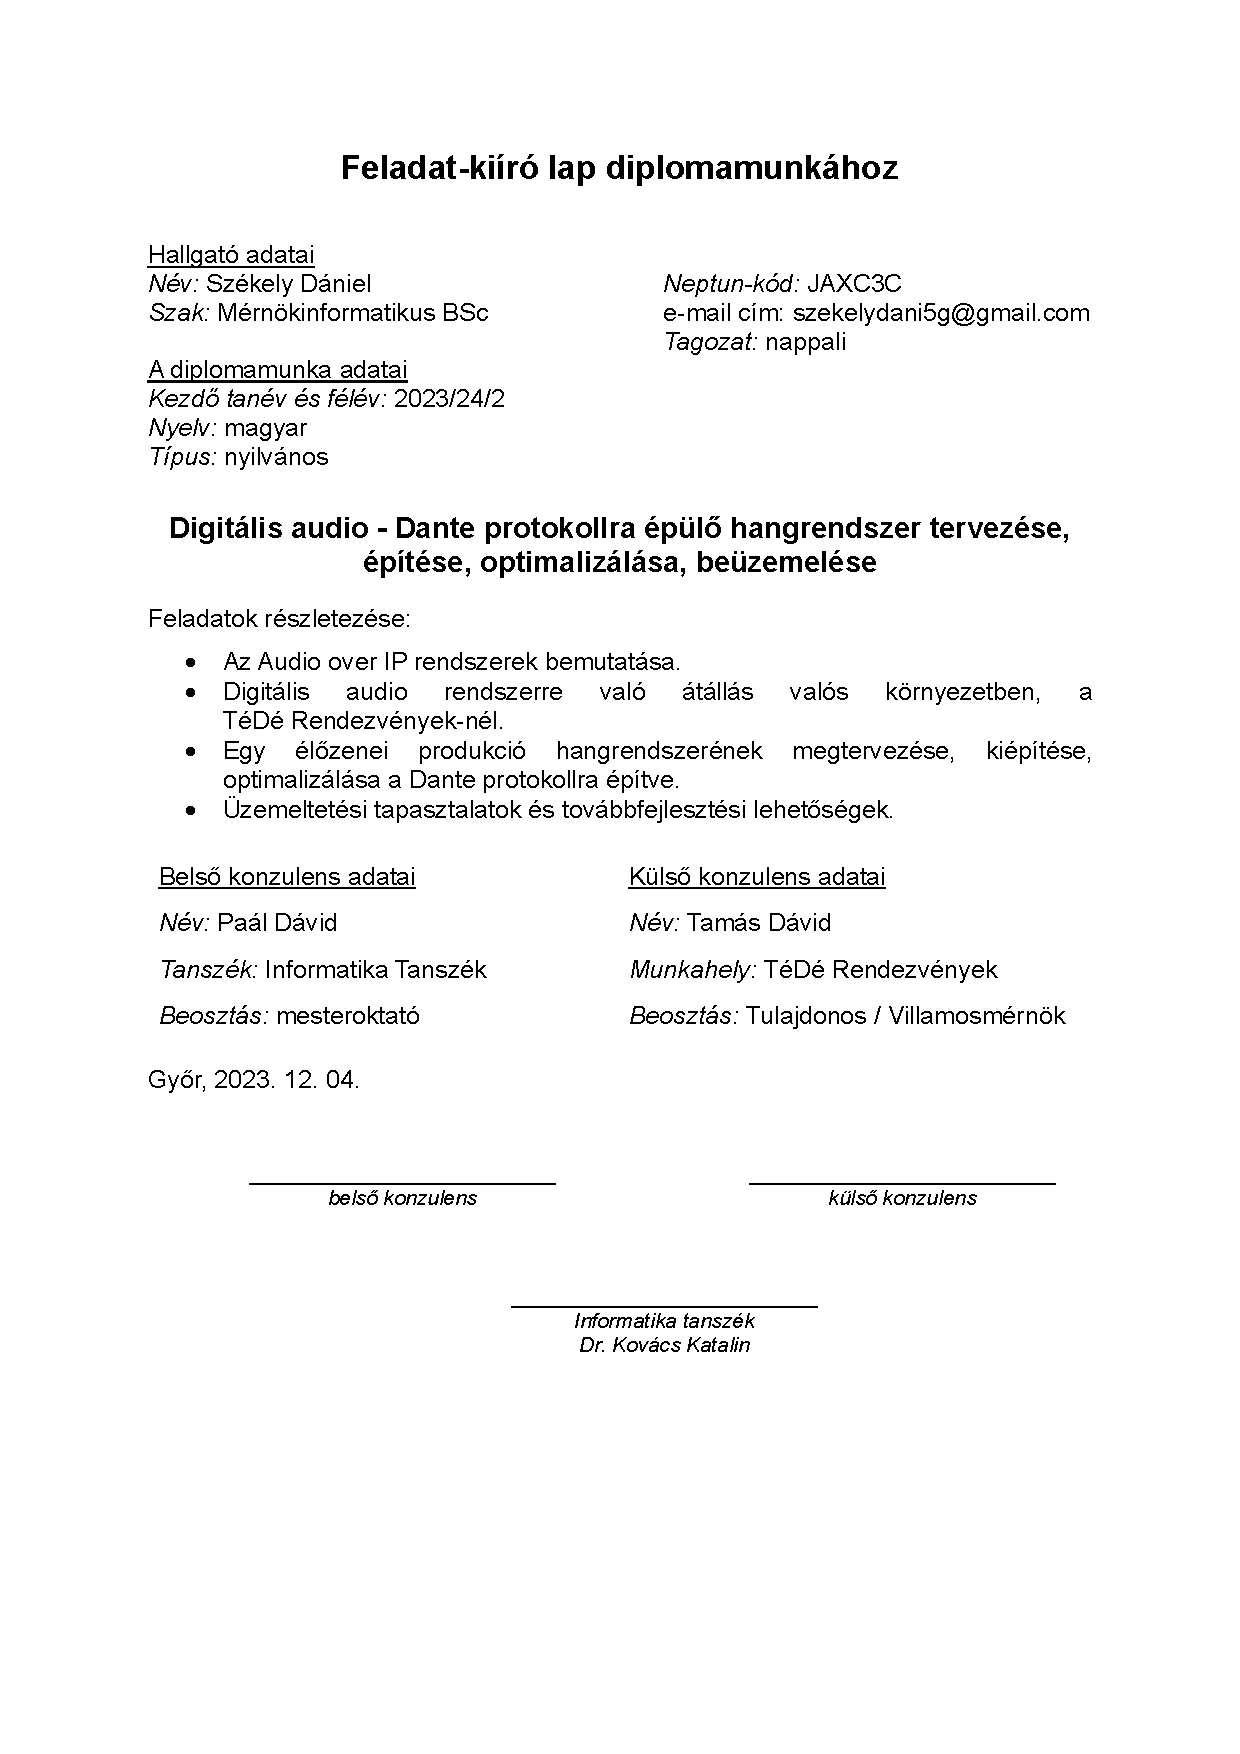
\includepdf{figures/start.pdf}

% Képfájlokhoz
\includegraphics*[width=\linewidth]{figures/start.png}


% Nyilatkozat és Kivonat
%~~~~~~~~~~~~~~~~~~~~~~~~~~~~~~~~~~~~~~~~~~~~~~~~~~~~~~~~~~~~~~~~~~~~~~~~~~~~~~~~~~~~~~
\selectlanguage{magyar}
\enfalse
\hutrue
\pagenumbering{gobble}
%--------------------------------------------------------------------------------------
% Nyilatkozat
%--------------------------------------------------------------------------------------
\chapter*{Nyilatkozat}

\noindent
Alulírott, \textbf{\szerzoVezeteknev{} \szerzoKeresztnev{} (\szerzoNeptun)}, \szak{} szakos hallgató kijelentem, hogy a \textit{\cim} című \MakeLowercase{\doktipus{}} feladat kidolgozása a saját munkám, abban csak a megjelölt forrásokat, és a megjelölt mértékben használtam fel, az idézés szabályainak megfelelően, a hivatkozások pontos megjelölésével.

\setlength\parskip{\baselineskip}

\noindent
Eredményeim saját munkán, számításokon, kutatáson, valós méréseken alapulnak, és a legjobb tudásom szerint hitelesek.

\vspace*{24pt}
\begin{multicols}{2}
	\noindent
	Győr, \emitdate{b}{\today}

	\columnbreak
	\noindent
	\makebox[7cm][c]{\rule{6cm}{.4pt}}\\
	\makebox[7cm][c]{\emph{\szerzoVezeteknev{} \szerzoKeresztnev}}\\
	\makebox[7cm]{hallgató}
\end{multicols}

\thispagestyle{empty}

\vfill
\clearpage
\thispagestyle{empty} % an empty page

\selectthesislanguage
 % ez legenerálódik magától a fentebb megadott adatok alapján
\pagenumbering{roman}
\setcounter{page}{1}

\selecthungarian

%----------------------------------------------------------------------------
% Kivonat Magyarul 
%----------------------------------------------------------------------------
\chapter*{Kivonat}
% TODO: Távolítsd el a megjegyzést, ha mégis szeretnéd, hogy bekerüljön a tartalomjegyzékbe
%\addcontentsline{toc}{chapter}{Kivonat}

Szakdolgozatom célja egy élőzenei produkció hangrendszerének megtervezése, 
kiépítése, optimalizálása és beüzemelése, mely a Dante protokollra 
építkezik. Az Audio over IP rendszerek, különösen a Dante hálózatok, 
lehetőséget nyújtanak a hagyományos analóg hangrendszerekhez 
képest gyorsabb, megbízhatóbb és skálázhatóbb megoldások alkalmazására. 

Az 1. fejezet bevezeti a szakdolgozat témáját és eredetét,
miért is ezt a témát választottam.

A 2. fejezet az alapvető hangtechnikai fogalmakat és rendszereket 
mutatja be, beleértve az analóg és digitális hangrendszerek 
közötti eltéréseket. 

A 3. fejezet célja, hogy alaposan bemutassa a digitális audió 
rendszerek alapjait és a Dante protokoll technikai részleteit. 
Ebben a részben többek között bemutatásra kerülnek az IP-címek kiosztásának módszerei, 
a hálózati topológiák kialakítása, 
valamint a különböző hálózati eszközök, mint például a switchek szerepei.

A 4. fejezet a tervezési és telepítési folyamatot tárgyalja, 
különös figyelmet szentelve a felhasznált eszközöknek, 
mint például a hangprocesszorok, végerősítők és 
hangszórók. 
A telepítés során a Dante alapú hálózat  kiépítése mellett kiemelten
foglalkozom a hangminőség optimalizálásával. A valós környezetben 
végzett tesztelés során a rendszer megbízhatóságát és 
rugalmasságát is értékelem.

Az 5. fejezet a telepítés utáni üzemeltetési tapasztalatokkal 
foglalkozik. Részletesen bemutatom a rendszer integrálását a 
TéDé Rendezvények egy élőzenei produkcióján, ahol 
valós időben teszteltem a Dante hálózat teljesítményét. 
Itt tárgyalom a hangrendszer és a vezérlőrendszerek 
integrációjának fontosságát, valamint az előadás közben 
tapasztalt akusztikai és hálózati kihívások kezelését. 
Az eredmények alapján további fejlesztési lehetőségeket 
javaslok, melyek még tovább növelhetik a rendszer teljesítményét és rugalmasságát.

Az általam bemutatott rendszer lényeges előnyöket nyújt egy analóg 
hangrendszerrel szemben.
Az üzemeltetési tapasztalatok azt igazolják, hogy 
az Audio over IP technológiák, különösen a Dante, 
stabil, skálázható és megbízható megoldást 
kínál a modern élőzenei produkciók számára.


\vfill
\selectenglish


%----------------------------------------------------------------------------
% Abstract in English
%----------------------------------------------------------------------------
\chapter*{Abstract}
% TODO: Távolítsd el a megjegyzést, ha mégis szeretnéd, hogy bekerüljön a tartalomjegyzékbe
%\addcontentsline{toc}{chapter}{Abstract}

The goal of my thesis is to design, build, optimize, and commission a sound system for 
a live music production based on the Dante protocol. Audio over IP systems, particularly 
Dante networks, offer faster, more reliable, and scalable solutions compared to traditional analog sound systems.

Chapter 1 introduces the topic and origin of the thesis, explaining why I chose this subject.

Chapter 2 presents the fundamental concepts and systems of sound technology, including 
the differences between analog and digital sound systems.

The purpose of Chapter 3 is to provide an in-depth overview of the fundamentals of 
digital audio systems and the technical details of the Dante protocol. This chapter 
includes topics such as methods for assigning IP addresses, designing network 
topologies, and the roles of various network devices, such as switches.

Chapter 4 discusses the design and installation process, with special emphasis on 
the equipment used, such as sound processors, amplifiers, and speakers. 
In addition to building the Dante-based network, I focus on optimizing sound quality 
during installation. During real-world testing, I evaluate the reliability and flexibility of the system.

Chapter 5 covers the operational experiences after installation. It details the 
integration of the system into a live music production by TéDé Rendezvények, where 
I tested the performance of the Dante network in real-time. 
This section highlights the importance of integrating the sound system with 
control systems and addresses the acoustic and network challenges encountered 
during the performance. Based on the results, I propose further development 
opportunities to enhance the system's performance and flexibility.

The system I present offers significant advantages over analog sound systems. 
Operational experiences confirm that Audio over IP technologies, particularly 
Dante, provide a stable, scalable, and reliable solution for modern live music productions.

\vfill
\selectthesislanguage

\newcounter{romanPage}
\setcounter{romanPage}{\value{page}}
\stepcounter{romanPage} %TODO ezt át kell írnod

% Tartalomjegyzék
%~~~~~~~~~~~~~~~~~~~~~~~~~~~~~~~~~~~~~~~~~~~~~~~~~~~~~~~~~~~~~~~~~~~~~~~~~~~~~~~~~~~~~~
\tableofcontents\vfill

% A dolgozat lényegi része
%~~~~~~~~~~~~~~~~~~~~~~~~~~~~~~~~~~~~~~~~~~~~~~~~~~~~~~~~~~~~~~~~~~~~~~~~~~~~~~~~~~~~~~
\pagenumbering{arabic}

%TODO készítsd el a saját munkád
%----------------------------------------------------------------------------
\chapter{\bevezetes}
%----------------------------------------------------------------------------

%----------------------------------------------------------------------------
\section{A kezdetek}
%----------------------------------------------------------------------------

Kisgyermek koromtól kezdve érdekelnek a hangtechnikához fűződő eszközök és azok elméleti-gyakorlati működése. Első élményeim egyike közé tartozik az, amikor
szüleim egy új fajta rádiólejátszót vásároltak otthonra, amelyen már nem csak a rádióadásokat lehetett hallgatni, hanem lejátszhatóak voltak kazetták is.
A készüléket akkoriban jobban tudtam kezelni gyermekként, mint a szüleim, egyértelmű volt már akkoriban is, a technika és a zene iránti érdeklődésem.
Ezek után általános iskolában a fizika tanárommal együtt kezdük el a sulirádió működtetését, amelynek a telepítési részében is részt vettem, mivel azelőtt
csak egyszerű csengők voltak felszerelve az épületben. Szükség volt hangsugárzókra, erősítőkre, mikrofonokra, és egyéb kiegészítőkre. A rádió működtetése
is az én feladatom lett két másik barátommal együtt, az iskolával kapcsolatos híreket és információkat mondtuk be rövid szünetekben, a hosszabb szünetekben pedig zenéket játszottunk.
Mindeközben zeneiskolába is beiratkoztam, ahol ütőhangszeresként tanultam egészen egyetemi tanulmányaim kezdetéig. A több mint tíz év alatt, sok új ismeretet és tapasztalatot szereztem,
amit a későbbiekben mint zenész, mint hangosító tudtam hasznosítani. Megismerkedtem a különböző zenei stílusok egyedi hangzásvilágával, ami a későbbiekben a hangosításban is nagy segítségemre volt.
Középiskolai tanulmányaim alatt kezdtem el komolyabban foglalkozni a hangtechinka világával komolyabb szinten. 
A fizika tanárommal ugyanis korábban nem csak a sulirádiót működtettük, hanem az összes sulibulit és rendezvényt a faluban mi szolgáltuk ki technikailag.
Ezért mivel már középiskolába jártam, a későbbiekben egy feltörekvő fiatalos és modern gondolkodású magánvállalkozáshoz ajánlott be engem, mivel a fiatal és motivált munkaerőt kerestek. (TéDé Rendezvények)
Már az első munkalehetőségnél éreztem, hogy ez egy nagyon jó lehetőség számomra, mindenképpen szeretnék ebben a szakmában dolgozni.
A cég fő profilja a hangrendszerek kiépítése és üzemeltetése volt, de későbbiekben már a fénytechnikával és színpadtechnikával is el kezdtünk foglalkozni. 
Ettől kezdve kezdtem el aktívan dolgozni a rendezvényiparban a hangrendszerek világában. Az évek során egyre több tapasztalatot
szereztem. Évente több mint száz rendezvényen tudtam folyamatosan fejlődni, rutint és ismerettséget szerezni a szakmában.

\subsection{Téma választás}

A hangrendszerek világa az elmúlt években nagy változáson ment keresztül. A digitális technika térhódítása a hangtechnikában is megjelent, és egyre több fajta megoldás jelent meg a piacon.
A digitális fejlesztésekből mi sem szerettünk volna kimaradni, hogy hangtechnikai apparátusunk korszerű és versenyképes maradjon.
Ekkor jött a fejlesztési ötlet, egy olyan rendszert tervezni, amely teljes mértékben digitális alapokra helyezi a jelenlegi hibrid megoldásunkat. A cégvezetőtől azt a feladatot kaptam,
hogy tervezzek egy olyan rendszert, amely megoldja a jelenlegi hibrid rendszerünk teljes digitális megoldásra való cseréjét. 
Az alapvető szempontok közé tartozott, hogy a rendszer legyen könnyen skálázható, és bővíthető, valamint a jelenlegi rendszert minden tekintetben felülmúlja.
Első lépésben a különböző Audio over IP protokollok közül kellett választanom,
amely a leginkább megfelel a rendszerünk igényeinek. Ehhez a piacon lévő protokollokat kellett megvizsgálnom, és a legjobb megoldást választani. 
Szakdolgozatomban sok idegen nyelvű szóra nincsen megfelelő és pontos fordítás ami teljes mértékben tükrözné az adott kifejezés jelentését.
A továbbiakban ebből kifolyólag feltételezve azt, hogy az olvasó tisztában van a szakmai terminológiával angolul fogom említeni a szakmai kifejezéseket.
Ezek a kifejezések megjelenhetnek írt szövegként és ábrás illusztrációkban is.

%----------------------------------------------------------------------------
\chapter{A dolgozatról}
%----------------------------------------------------------------------------

%----------------------------------------------------------------------------
\section{A dolgozat célja}
%----------------------------------------------------------------------------
A szakdolgozat és a diplomamunka célja annak bizonyítása, hogy a jelölt önálló mérnöki munkára képes. Az elkészített mű tehát saját alkotómunkát kell, hogy bizonyítson!

%----------------------------------------------------------------------------
\section{A dolgozat felépítése}
%----------------------------------------------------------------------------
A dolgozat sorszámozott fejezetekből, illetve alfejezetekből áll. A tartalomjegyzék a sablon szerint a dolgozat elején legyen. A dolgozat néhány oldalas bevezetővel kezdődjék, amely bemutatja a feldolgozott szakterületet, ha szükséges történelmi utalásokat is tehet, s a jelölt itt jusson el a megoldandó probléma világos, tényszerű megfogalmazásához, s vázolja fel, hogy azt milyen módon oldotta meg. Ha szükséges, röviden bemutathatja a céget, ahol a munkát végezte, méltathatja a felvetett probléma időszerűségét, a megoldás korszerűségét. A bevezető célja, hogy a bíráló, vagy az olvasó el tudja helyezni az elkészített munkát a szakmán belül. A dolgozat fejezeteinek számozását a Bevezető fejezettel kezdje.

A felhasznált szakirodalomnak a jelölt által történő feldolgozása és bemutatása rendkívül fontos, hiszen a munkát arra alapozva készíti el. Szükséges tehát egy olyan fejezet megírása is (amely rendre a bevezetést követi), amelyben a jelölt a szakirodalomra (szakkönyvek, szakcikkek, tankönyvek) hivatkozva összegzi a már ismert tényeket, eredményeket és összefüggéseket. A felhasznált irodalom feldolgozásáról szóló fejezet ne a jól ismert tananyag ismétlése legyen! Törekedjen arra, hogy a fejezet áttekintése után az olvasó elegendő ismerettel rendelkezzen ahhoz, hogy a jelölt saját munkáját megértse. Használja a könyvtárat, s válogasson az interneten közzétett anyagok között, de kerülje a kétes eredetű forrásokat! Ez a fejezet kb. 10-15 oldal terjedelmű legyen.

A következő fejezet az elvégzett munkát hivatott bemutatni, s így a terjedelme is nagyobb kell, hogy legyen. A dolgozat írásakor ezen fejezetben nyugodtan használhat egyes szám első személyt (pl. megoldottam, megterveztem stb.), hiszen a munka a sajátja. A fejezetet célszerűen a feladat részletes leírásával kezdje, térjen ki minden lényeges momentumra. Gyakran előfordul, hogy a feladat egy meglevő rendszer átalakítása, bővítése. Ilyenkor a meglevő rendszer ismertetése a fejezet elején történjen meg, a változtatások bemutatása, a tervezés menete, az elvégzett lépések indoklása stb. pedig a fejezet fő súlypontját alkossák. Ebben a fejezetben fotókon, ábrákon, grafikonokon, képleteken keresztül érthetően, világosan mutassa be, hogy mi a saját, önálló tevékenysége, mit és hogyan oldott meg, azokból milyen eredmények születtek. A fejezet végén elemezze az elkészült munkát. Ez a fejezet legyen kb. 30-40 oldal, s ez legyen a dolgozat hangsúlyos része. Amennyiben munkája több, határozottan elkülönülő tevékenységből állt, ez a rész több fejezetre is tagolható.

A dolgozatot az összefoglalás zárja. Itt múlt időben a szerző röviden ismételje meg, hogy mit és hogy valósított meg. Ebben a rövid, egy-két oldalas fejezetben a jelölt rámutathat a még megoldásra váró kérdésekre, esetleges jövőbeni tervekre, feladatokra. Írja le tapasztalatait, következtetéseit.

A következő szakasz az irodalomjegyzék, amelynek formája kötött. A Tanszék megkötése, hogy az internetes források száma nem érheti el a teljes irodalmi hivatkozások számának 30\%-át, továbbá internetes forrás megjelölésekor kötelező a honlap utolsó látogatásának időpontját is megadni! Az irodalmi hivatkozásokat a szövegben a megfelelő helyen jelölni kell. A szerzők nevét mindenütt “Családnév, X.” formában kell megadni, ahol X. a szerző keresztnevének (keresztneveinek) kezdőbetűje. Magyar cikk esetén a vessző a családnév és a keresztnév kezdőbetűje közt elhagyható. Ha az egyértelműség megkívánja, a keresztnév kiírható teljesen is. Az irodalmi hivatkozások \ref{sec:HowtoReference} fejezetben bővebben kitérünk.

%----------------------------------------------------------------------------
\section{Formai követelmények}
%----------------------------------------------------------------------------
A \LaTeX{} sablon előnye, hogy ezzel nem kell foglalkoznod. Ha rendeltetésszerűen használod a sablont, akkor formai szempontból a dolgozat megfelelő lesz.

%TODO@FMA: SZE követelmenyek
%----------------------------------------------------------------------------
\section{A dolgozat nyelve}
%----------------------------------------------------------------------------
Mivel Magyarországon a hivatalos nyelv a magyar, ezért alapértelmezésben magyarul kell megírni a dolgozatot. Aki külföldi posztgraduális képzésben akar részt venni, nemzetközi szintű tudományos kutatást szeretne végezni, vagy multinacionális cégnél akar elhelyezkedni, annak célszerű angolul megírnia diplomadolgozatát. Mielőtt a hallgató az angol nyelvű verzió mellett dönt, erősen ajánlott mérlegelni, hogy ez mennyi többletmunkát fog a hallgatónak jelenteni fogalmazás és nyelvhelyesség terén, valamint -- nem utolsó sorban -- hogy ez mennyi többletmunkát fog jelenteni a konzulens illetve bíráló számára. Egy nehezen olvasható, netalán érthetetlen szöveg teher minden játékos számára.

%TODO@FMA: SZE követelmenyek
%----------------------------------------------------------------------------
\section{A dokumentum nyomdatechnikai kivitele}
%----------------------------------------------------------------------------
A dolgozatot A4-es fehér lapra nyomtatva, 2,5 centiméteres margóval (+1~cm kötésbeni), 11--12 pontos betűmérettel, talpas betűtípussal és másfeles sorközzel célszerű elkészíteni.

Annak érdekében, hogy a dolgozat külsőleg is igényes munka benyomását keltse, érdemes figyelni az alapvető tipográfiai szabályok betartására~\cite{Jeney}.

%----------------------------------------------------------------------------
\chapter{\LaTeX-eszközök}
\label{sec:LatexTools}
%----------------------------------------------------------------------------
\section{A szerkesztéshez használatos eszközök}
%----------------------------------------------------------------------------
Ez a sablon TeXstudio 2.8.8 szerkesztővel készült. A TeXstudio egy platformfüggetlen, Windows, Linux és Mac OS alatt is elérhető \LaTeX-szerkesztőprogram számtalan hasznos szolgáltatással (\refstruc{fig:TeXstudio}). A szoftver ingyenesen letölthető\footnote{A TeXstudio hivatalos oldala: \url{http://texstudio.sourceforge.net/}}.

\begin{figure}[!ht]
\centering
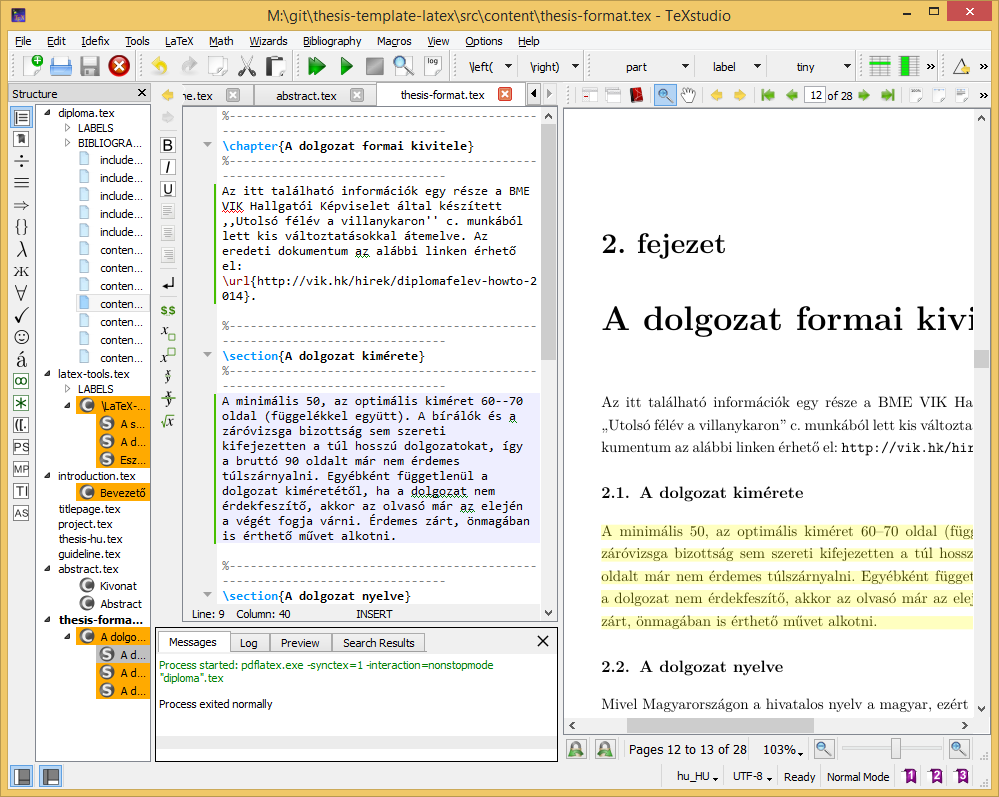
\includegraphics[width=150mm, keepaspectratio]{figures/TeXstudio.png}
\caption{A TeXstudio \LaTeX-szerkesztő.}
\label{fig:TeXstudio}
\end{figure}

A TeXstudio telepítése után érdemes még letölteni a magyar nyelvű helyesírásellenőrző-szótárakat hozzá. A TeXstudio az OpenOffice-hoz használatos formátumot tudja kezelni. A TeXstudio beállításainál a \texttt{General} fülön a \texttt{Dictionaries} résznél tudjuk megadni, hogy melyik szótárat használja.

Egy másik használható Windows alapú szerkesztőprogram a LEd\footnote{A LEd hivatalos oldala: \url{http://www.latexeditor.org/}} (LaTeX Editor), a TeXstudio azonban stabilabb, gyorsabb, és jobban használható.

Természetesen nem kötelező IDE használata, a legnépszerűbb szövegszerkesztők rendelkeznek mind Git, mind \LaTeX{} kiegészítő csomagokkal:

\begin{itemize}
    \item \textbf {Sublime Text 3}: gitsavvy + LatexTools
    \item \textbf {Visual Studio Code}: built in git + gitlens + LatexWorkshop
\end{itemize} 

Egy másik, modern alternatíva az \textit{Overleaf}. A \ref{fig:overleaf}. ábrán látható webes felület bárhonnan elérhető és szinte többet tud mint az offline környezetek:

\begin{itemize}
    \item Jól működő autocomplete
    \item Git integráció, GitHub connection
    \item Magyar spellcheck
    \item Többféle fordító, jól látható compiler log
    \item Nagyon egyszerű használni bármilyen eszközön, nem kell foglalkozni a \LaTeX{} fordítók telepítésével
\end{itemize}

\begin{figure}[!ht]
    \centering
    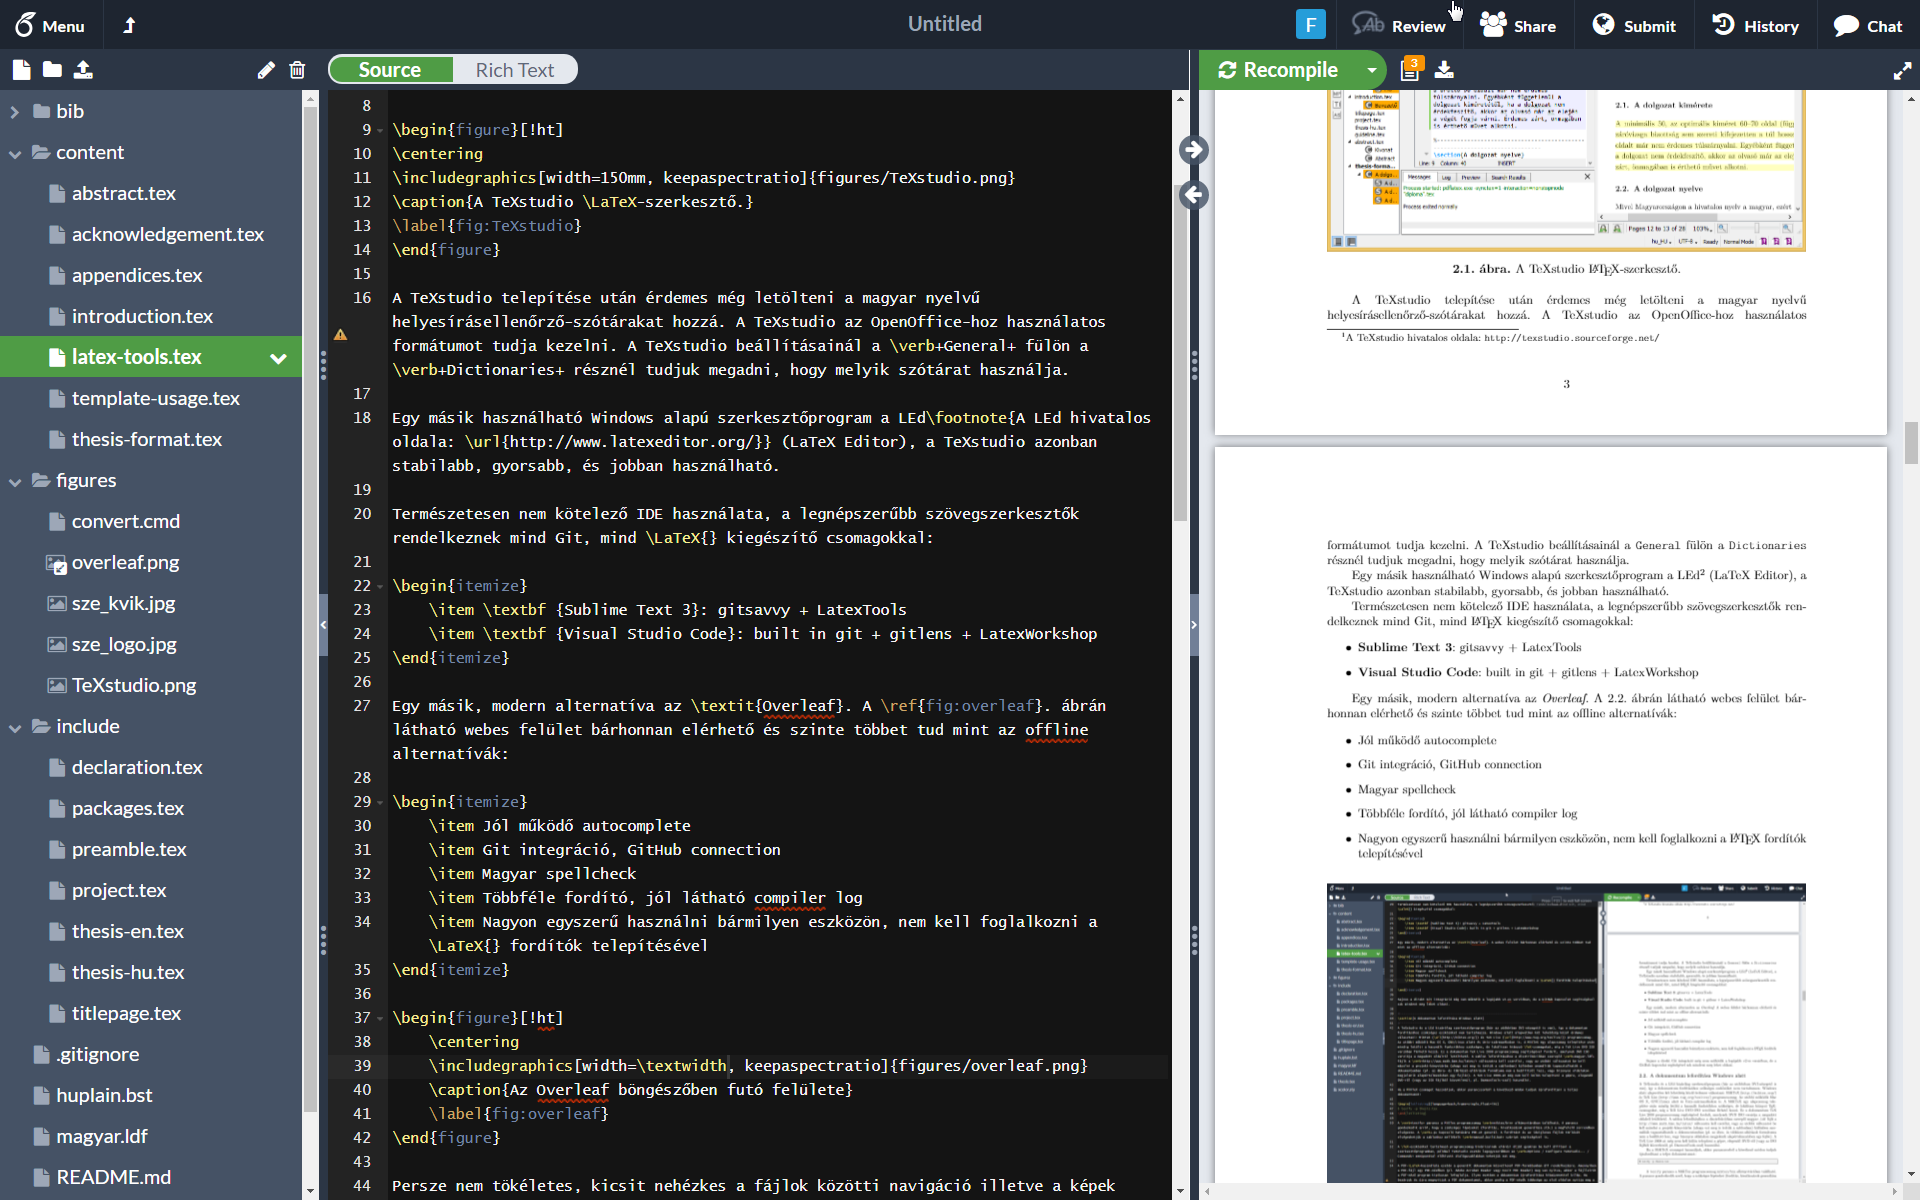
\includegraphics[width=\textwidth, keepaspectratio]{figures/overleaf.png}
    \caption{Az Overleaf böngészőben futó felülete}
    \label{fig:overleaf}
\end{figure}

Persze nem tökéletes, kicsit nehézkes a fájlok közötti navigáció illetve a képek beillesztése, de az, hogy bármilyen gépről lehet használni anélkül hogy felkonfigurálnánk a szokásos \LaTeX{} környezetünket, hatalmas előny. Sajnos a direkt Git integráció még nem működik a legújabb v2-es verzióban, de a GitHub kapcsolat segítségével sok mindent meg lehet oldani.

%----------------------------------------------------------------------------
\section{A dokumentum lefordítása Windows alatt}
%----------------------------------------------------------------------------
A TeXstudio és a LEd kizárólag szerkesztőprogram (bár az utóbbiban DVI-nézegető is van), így a dokumentum fordításához szükséges eszközöket nem tartalmazza. Windows alatt alapvetően két lehetőség közül érdemes választani: MiKTeX (\url{http://miktex.org/}) és TeX Live (\url{http://www.tug.org/texlive/}) programcsomag. Az utóbbi működik Mac OS X, GNU/Linux alatt és Unix-származékokon is. A MiKTeX egy alapcsomag telepítése után mindig letölti a használt funkciókhoz szükséges, de lokálisan hiányzó \TeX-csomagokat, míg a TeX Live DVD ISO verzóban férhető hozzá. Ez a dokumentum TeX Live 2008 programcsomag segítségével fordult, amelynek DVD ISO verziója a megadott oldalról letölthető. A sablon lefordításához a disztribúcióban szereplő \verb+magyar.ldf+ fájlt a \verb+http://www.math.bme.hu/latex/+ változatra kell cserélni, vagy az utóbbi változatot be kell másolni a projekt-könyvtárba (ahogy ezt meg is tettük a sablonban) különben anomáliák tapasztalhatók a dokumentumban (pl. az ábra- és táblázat-aláírások formátuma nem a beállított lesz, vagy bizonyos oldalakon megjelenik alapértelmezésben egy fejléc). A TeX Live 2008-at még nem kell külön telepíteni a gépre, elegendő DVD-ről (vagy az ISO fájlból közvetlenül, pl. DaemonTools-szal) használni.

Ha a MiKTeX csomagot használjuk, akkor parancssorból a következő módon tudjuk újrafordítani a teljes dokumentumot:

\begin{lstlisting}[language=bash,frame=single,float=!ht]
$ texify -p thesis.tex
\end{lstlisting}

A \verb+texify+ parancs a MiKTex programcsomag \verb+miktex/bin+ alkönyvtárában található. A parancs gondoskodik arról, hogy a szükséges lépéseket (fordítás, hivatkozások generálása stb.) a megfelelő sorrendben elvégezze. A \verb+-p+ kapcsoló hatására PDF-et generál. A fordítást és az ideiglenes fájlok törlését elvégezhetjük a sablonhoz mellékelt \verb+manual_build.bat+ szkript segítségével is.

A \TeX-eszközöket tartalmazó programcsomag binárisainak elérési útját gyakran be kell állítani a szerkesztőprogramban, például TeXstudio esetén legegyszerűbben az \verb+Options / Configure TeXstudio... / Commands+ menüponttal előhívott dialógusablakban tehetjük ezt meg.

A PDF-\LaTeX~használata esetén a generált dokumentum közvetlenül PDF-formátumban áll rendelkezésre. Amennyiben a PDF-fájl egy PDF-nézőben (pl. Adobe Acrobat Reader vagy Foxit PDF Reader) meg van nyitva, akkor a fájlleírót a PDF-néző program tipikusan lefoglalja. Ilyen esetben a dokumentum újrafordítása hibaüzenettel kilép. Ha bezárjuk és újra megnyitjuk a PDF dokumentumot, akkor pedig a PDF-nézők többsége az első oldalon nyitja meg a dokumentumot, nem a legutóbb olvasott oldalon. Ezzel szemben például az egyszerű és ingyenes \textcolor{blue}{Sumatra PDF} nevű program képes arra, hogy a megnyitott dokumentum megváltozását detektálja, és frissítse a nézetet az aktuális oldal megtartásával.

%----------------------------------------------------------------------------
\section{Eszközök Linuxhoz}
%----------------------------------------------------------------------------
Linux operációs rendszer alatt is rengeteg szerkesztőprogram van, pl. a KDE alapú Kile jól használható. Ez ingyenesen letölthető, vagy éppenséggel az adott Linux-disztribúció eleve tartalmazza, ahogyan a dokumentum fordításához szükséges csomagokat is. Az Ubuntu Linux disztribúciók alatt például legtöbbször a \verb+texlive-*+ csomagok telepítésével használhatók a \LaTeX-eszközök. A jelen sablon fordításához szükséges csomagok (kb. 0,5 GB) az alábbi paranccsal telepíthetők:

\begin{lstlisting}[language=bash,morekeywords={sudo,apt\-get},alsoletter={-},breaklines=true]
$ sudo apt-get install texlive-latex-extra texlive-fonts-extra texlive-fonts-recommended texlive-xetex texlive-science
\end{lstlisting}

Amennyiben egy újabb csomag hozzáadása után hiányzó fájlra utaló hibát kapunk a fordítótól, telepítenünk kell az azt tartalmazó TeX Live csomagot. Ha pl. a \verb+bibentry+ csomagot szeretnénk használni, futtassuk az alábbi parancsot:

\begin{lstlisting}[language=bash,morekeywords={apt\-cache},alsoletter={-},breaklines=true]
$ apt-cache search bibentry
texlive-luatex - TeX Live: LuaTeX packages
\end{lstlisting}

Majd telepítsük fel a megfelelő TeX Live csomagot, jelen esetben a `texlive-lualatex`-et. (Egy LaTeX csomag több TeX Live csomagban is szerepelhet.)

Ha gyakran szerkesztünk más \LaTeX dokumentumokat is, kényelmes és biztos megoldás a teljes TeX Live disztribúció telepítése, ez azonban kb. 4 GB helyet igényel.

\begin{lstlisting}[language=bash,morekeywords={sudo,apt\-get},alsoletter={-},breaklines=true]
sudo apt-get install texlive-full
\end{lstlisting}

% !TeX spellcheck = hu_HU
% !TeX encoding = UTF-8
% !TeX program = xelatex
%----------------------------------------------------------------------------
\chapter{A \LaTeX-sablon használata}
%----------------------------------------------------------------------------

Ebben a fejezetben röviden, implicit módon bemutatjuk a sablon használatának módját, ami azt jelenti, hogy sablon használata ennek a dokumentumnak a forráskódját tanulmányozva válik teljesen világossá. Amennyiben a szoftver-keretrendszer telepítve van, a sablon alkalmazása és a dolgozat szerkesztése \LaTeX-ben a sablon segítségével tapasztalataink szerint jóval hatékonyabb, mint egy WYSWYG (\emph{What You See is What You Get}) típusú szövegszerkesztő esetén (pl. Microsoft Word, OpenOffice).

%----------------------------------------------------------------------------
\section{Címkék és hivatkozások}
%----------------------------------------------------------------------------
A \LaTeX~dokumentumban címkéket (\verb+\label+) rendelhetünk ábrákhoz, táblázatokhoz, fejezetekhez, listákhoz, képletekhez stb. Ezekre a dokumentum bármely részében hivatkozhatunk, a hivatkozások automatikusan feloldásra kerülnek.

A sablonban makrókat definiáltunk a hivatkozások megkönnyítéséhez. Ennek megfelelően minden ábra (\emph{figure}) címkéje \verb+fig:+ kulcsszóval kezdődik, míg minden táblázat (\emph{table}), képlet (\emph{equation}), fejezet (\emph{section}) és lista (\emph{listing}) rendre a \verb+tab:+, \verb+eq:+, \verb+sec:+ és \verb+lst:+ kulcsszóval kezdődik, és a kulcsszavak után tetszőlegesen választott címke használható. Ha ezt a konvenciót betartjuk, akkor az előbbi objektumok számára rendre a \verb+\figref+, \verb+\tabref+, \verb+\eqref+, \verb+\sectref+ és \verb+\listref+ makrókkal hivatkozhatunk. A makrók paramétere a címke, amelyre hivatkozunk (a kulcsszó nélkül). Az összes említett hivatkozástípus, beleértve az \verb+\url+ kulcsszóval bevezetett web-hivatkozásokat is a  \verb+hyperref+\footnote{Segítségével a dokumentumban megjelenő hivatkozások nem csak dinamikussá válnak, de színezhetők is, bővebbet erről a csomag dokumentációjában találunk. Ez egyúttal egy példa lábjegyzet írására.} csomagnak köszönhetően aktívak a legtöbb PDF-nézegetőben, rájuk kattintva a dokumentum megfelelő oldalára ugrik a PDF-néző vagy a megfelelő linket megnyitja az alapértelmezett böngészővel. A \verb+hyperref+ csomag a kimeneti PDF-dokumentumba könyvjelzőket is készít a tartalomjegyzékből. Ez egy szintén aktív tartalomjegyzék, amelynek elemeire kattintva a nézegető behozza a kiválasztott fejezetet.

%----------------------------------------------------------------------------
\section{Ábrák és táblázatok}
%----------------------------------------------------------------------------
Használjunk vektorgrafikus ábrákat, ha van rá módunk. PDFLaTeX használata esetén PDF formátumú ábrákat lehet beilleszteni könnyen, az EPS (PostScript) vektorgrafikus képformátum beillesztését a PDFLaTeX közvetlenül nem támogatja (de lehet konvertálni, lásd később). Ha vektorgrafikus formában nem áll rendelkezésünkre az ábra, akkor a  veszteségmentes PNG, valamint a veszteséges JPEG formátumban érdemes elmenteni.  Figyeljünk arra, hogy ilyenkor a képek felbontása elég nagy legyen ahhoz, hogy nyomtatásban is megfelelő minőséget nyújtson (legalább 300 dpi javasolt). A dokumentumban felhasznált képfájlokat a dokumentum forrása mellett érdemes tartani, archiválni, mivel ezek hiányában a dokumentum nem fordul újra. Ha lehet, a vektorgrafikus képeket vektorgrafikus formátumban is érdemes elmenteni az újrafelhasználhatóság (az átszerkeszthetőség) érdekében.

Kapcsolási rajzok legtöbbször kimásolhatók egy vektorgrafikus programba (pl. CorelDraw) és onnan nagyobb felbontással raszterizálva kimenthatők PNG formátumban. Ugyanakkor kiváló ábrák készíthetők Microsoft Visio vagy hasonló program használatával is: Visio-ból az ábrák közvetlenül PDF-be is menthetők.

Lehetőségeink Matlab ábrák esetén:
\begin{itemize}
	\item Képernyőlopás (\emph{screenshot}) is elfogadható minőségű lehet a dokumentumban, de általában jobb felbontást is el lehet érni más módszerrel.
	\item A Matlab ábrát a \verb+File/Save As+ opcióval lementhetjük PNG formátumban (ugyanaz itt is érvényes, mint korábban, ezért nem javasoljuk).
	\item A Matlab ábrát az \verb+Edit/Copy figure+ opcióval kimásolhatjuk egy vektorgrafikus programba is és onnan nagyobb felbontással raszterizálva kimenthatjük PNG formátumban (nem javasolt).
	\item Javasolt megoldás: az ábrát a \verb+File/Save As+ opcióval EPS \emph{vektorgrafikus} formátumban elmentjük, PDF-be konvertálva beillesztjük a dolgozatba.
\end{itemize}
Az EPS kép az \verb+epstopdf+ programmal\footnote{a korábban említett \LaTeX-disztribúciókban megtalálható} konvertálható PDF formátumba. Célszerű egy batch-fájlt készíteni az összes EPS ábra lefordítására az alábbi módon (ez Windows alatt működik).
\begin{lstlisting}[language=]
@echo off
for %%j in (*.eps) do (
  echo converting file "%%j"
  epstopdf "%%j"
)
echo done .
\end{lstlisting}

Egy ilyen parancsfájlt (\verb+convert.cmd+) elhelyeztük a sablon \verb+figures\eps+ könyvtárába, így a felhasználónak csak annyi a dolga, hogy a \verb+figures\eps+ könyvtárba kimenti az EPS formátumú vektorgrafikus képet, majd lefuttatja a \verb+convert.cmd+ parancsfájlt, ami PDF-be konvertálja az EPS fájlt.

Ezek után a PDF-ábrát ugyanúgy lehet a dokumentumba beilleszteni, mint a PNG-t vagy a JPEG-et. A megoldás előnye, hogy a lefordított dokumentumban is vektorgrafikusan tárolódik az ábra, így a mérete jóval kisebb, mintha raszterizáltuk volna beillesztés előtt. Ez a módszer minden -- az EPS formátumot ismerő -- vektorgrafikus program (pl. CorelDraw) esetén is használható.

A képek beillesztésére \az+\refstruc{sec:LatexTools}ben mutattunk be példát (\refstruc{fig:TeXstudio}). Az előző mondatban egyúttal az automatikusan feloldódó ábrahivatkozásra is láthatunk példát. Több képfájlt is beilleszthetünk egyetlen ábrába. Az egyes képek közötti horizontális és vertikális margót metrikusan szabályozhatjuk (\refstruc{fig:HVSpaces}). Az ábrák elhelyezését számtalan tipográfiai szabály egyidejű teljesítésével a fordító maga végzi, a dokumentum írója csak preferenciáit jelezheti a fordító felé (olykor ez bosszúságot is okozhat, ilyenkor pl. a kép méretével lehet játszani).

Ne felejtsük, hogy az SZE-GVIK szabályai szerint a nem saját magunk által készített ábrák forrását meg kell jelölni. Ennek a megkönnyítésére készült a \texttt{figsource} parancs aminek a használata a \ref{lst:figsourceExample}. kód részletben látható.

\begin{lstlisting}[language=tex,caption=Példa \texttt{figsource} használatára,label=lst:figsourceExample]
\begin{figure}
    \centering
    \includegraphics[width=67mm, keepaspectratio]{figures/peldaabra.png}
    \caption{James Clerk Maxwell}
    \label{fig:exampleFigure}
    \figsource{https://itsinterestingdotcom.files.wordpress.com/2016/02/james-clerk-maxwell.jpg}{9}{3}
\end{figure}
\end{lstlisting}

\begin{figure}
    \centering
    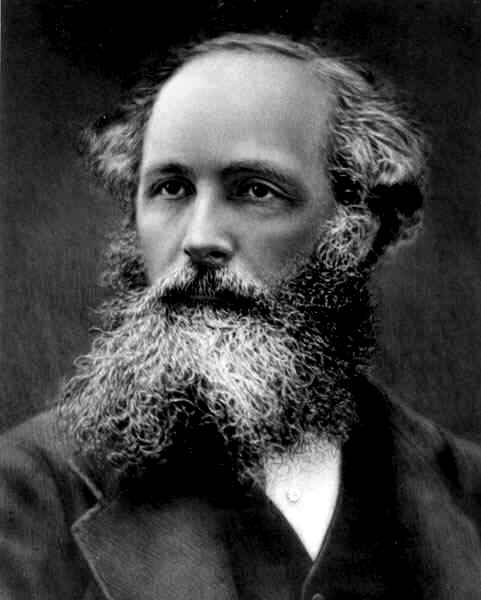
\includegraphics[width=67mm, keepaspectratio]{figures/james-clerk-maxwell.jpg}
    \caption{James Clerk Maxwell}
    \label{fig:exampleFigure}
    \figsource{https://itsinterestingdotcom.files.wordpress.com/2016/02/james-clerk-maxwell.jpg}{9}{3}
\end{figure}

\begin{figure}[!ht]
	\centering
	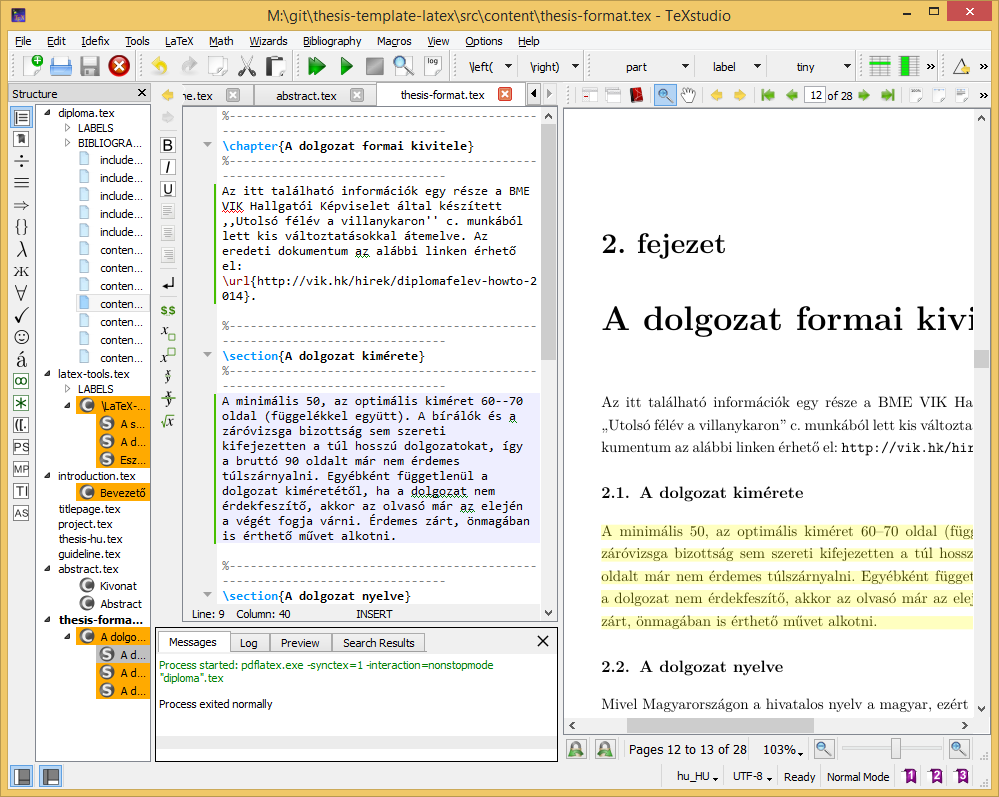
\includegraphics[width=67mm, keepaspectratio]{figures/TeXstudio.png}\hspace{1cm}
	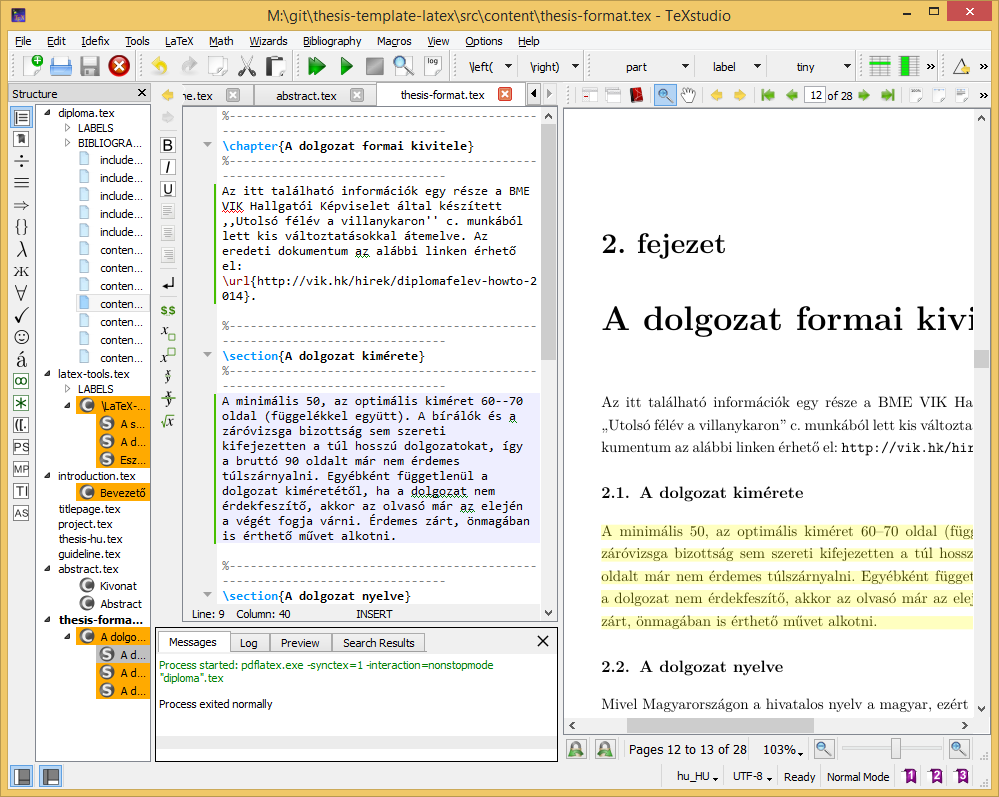
\includegraphics[width=67mm, keepaspectratio]{figures/TeXstudio.png}\\\vspace{5mm}
	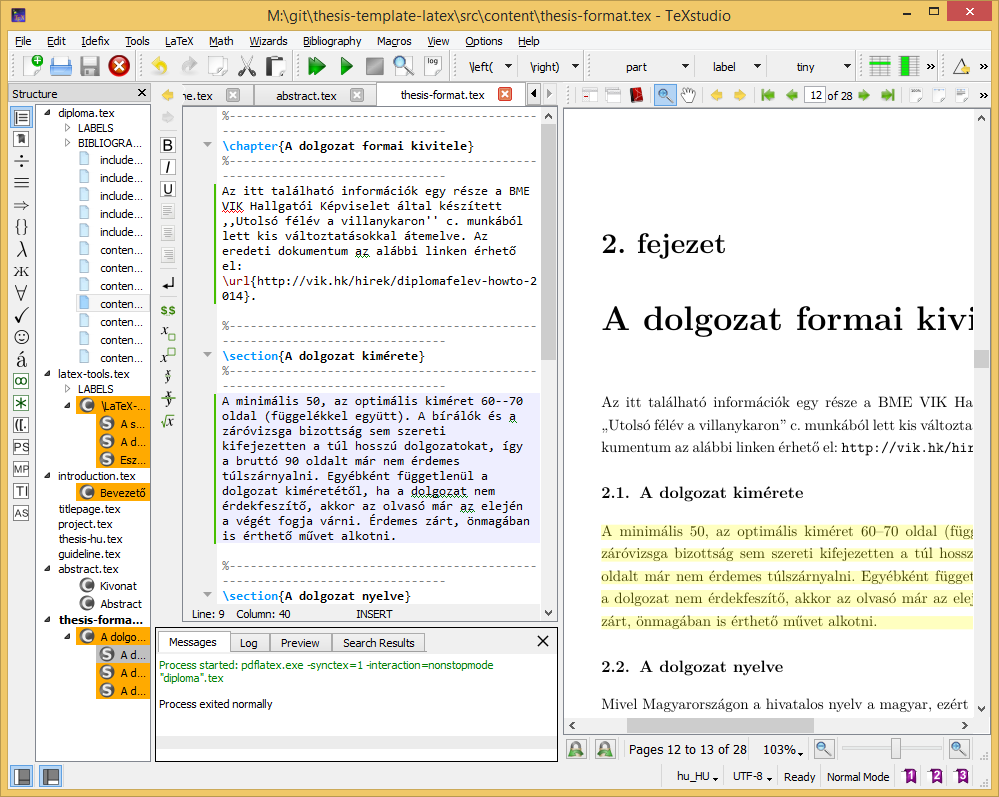
\includegraphics[width=67mm, keepaspectratio]{figures/TeXstudio.png}\hspace{1cm}
	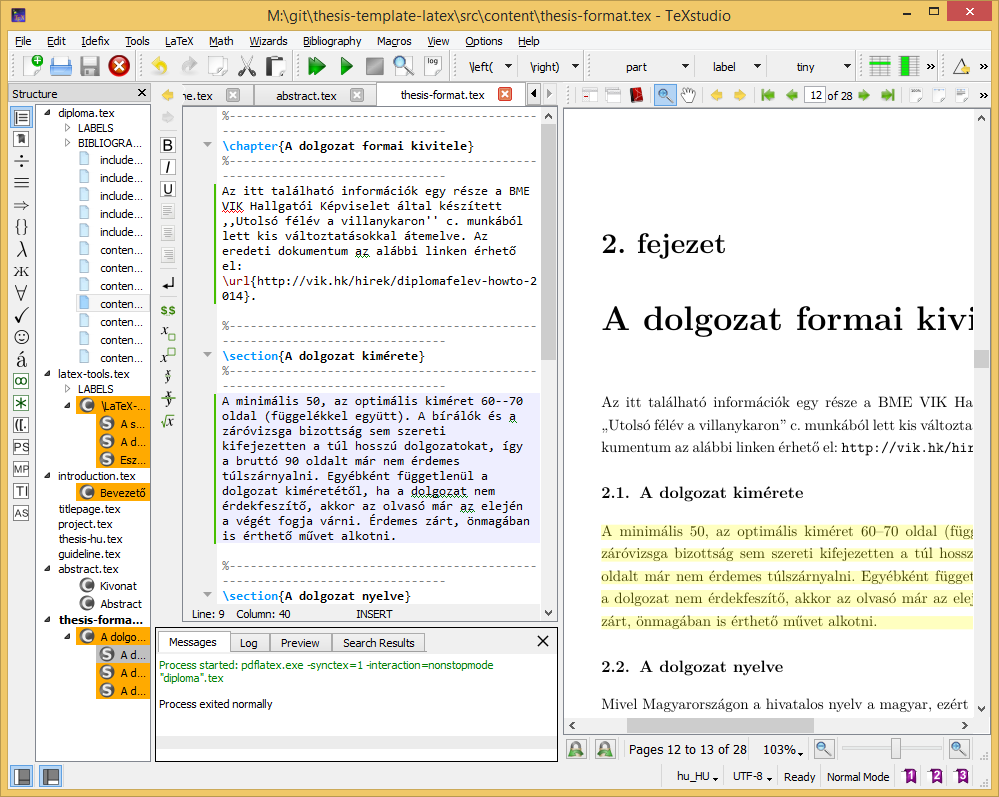
\includegraphics[width=67mm, keepaspectratio]{figures/TeXstudio.png}
	\caption{Több képfájl beillesztése esetén térközöket is érdemes használni.}
	\label{fig:HVSpaces}
\end{figure}

A táblázatok használatára \aref{tab:TabularExample}~táblázat mutat példát. A táblázatok formázásához hasznos tanácsokat találunk a \verb+booktabs+ csomag dokumentációjában.

\begin{table}[!ht]
	\footnotesize
	\centering
	\begin{tabular}{ l c c }
		\toprule
		Órajel & Frekvencia & Cél pin \\
		\midrule
		CLKA & 100 MHz & FPGA CLK0\\
		CLKB & 48 MHz  & FPGA CLK1\\
		CLKC & 20 MHz  & Processzor\\
		CLKD & 25 MHz  & Ethernet chip \\
		CLKE & 72 MHz  & FPGA CLK2\\
		XBUF & 20 MHz  & FPGA CLK3\\
		\bottomrule
	\end{tabular}
	\caption{Az órajel-generátor chip órajel-kimenetei.}
	\label{tab:TabularExample}
\end{table}


%----------------------------------------------------------------------------
\section{Felsorolások és listák}
%----------------------------------------------------------------------------
Számozatlan felsorolásra mutat példát a jelenlegi bekezdés:
\begin{itemize}
	\item \emph{első bajusz:} ide lehetne írni az első elem kifejését,
	\item \emph{második bajusz:} ide lehetne írni a második elem kifejését,
	\item \emph{ez meg egy szakáll:} ide lehetne írni a harmadik elem kifejését.
\end{itemize}

Számozott felsorolást is készíthetünk az alábbi módon:
\begin{enumerate}
	\item \emph{első bajusz:} ide lehetne írni az első elem kifejését, és ez a kifejtés így néz ki, ha több sorosra sikeredik,
	\item \emph{második bajusz:} ide lehetne írni a második elem kifejését,
	\item \emph{ez meg egy szakáll:} ide lehetne írni a harmadik elem kifejését.
\end{enumerate}
A felsorolásokban sorok végén vessző, az utolsó sor végén pedig pont a szokásos írásjel. Ez alól kivételt képezhet, ha az egyes elemek több teljes mondatot tartalmaznak.

Listákban a dolgozat szövegétől elkülönítendő kódrészleteket, programsorokat, pszeudo-kódokat jeleníthetünk meg (\ref{lst:Example}.~kódrészlet).
\begin{lstlisting}[language=tex,caption=A fenti számozott felsorolás \LaTeX-forráskódja,label=lst:Example]
\begin{enumerate}
	\item \emph{els(*@ő@*) bajusz:} ide lehetne írni az els(*@ő@*) elem kifejését,
	és ez a kifejtés így néz ki, ha több sorosra sikeredik,
	\item \emph{második bajusz:} ide lehetne írni a második elem kifejését,
	\item \emph{ez meg egy szakáll:} ide lehetne írni a harmadik elem kifejését.
\end{enumerate}
\end{lstlisting}
A lista keretét, háttérszínét, egész stílusát megválaszthatjuk. Ráadásul különféle programnyelveket és a nyelveken belül kulcsszavakat is definiálhatunk, ha szükséges. Erről bővebbet a \verb+listings+ csomag hivatalos leírásában találhatunk.

%----------------------------------------------------------------------------
\section{Képletek}
%----------------------------------------------------------------------------
Ha egy formula nem túlságosan hosszú, és nem akarjuk hivatkozni a szövegből, mint például a $e^{i\pi}+1=0$ képlet, \emph{szövegközi képletként} szokás leírni. Csak, hogy másik példát is lássunk, az $U_i=-d\Phi/dt$ Faraday-törvény a $\rot E=-\frac{dB}{dt}$ differenciális alakban adott Maxwell-egyenlet felületre vett integráljából vezethető le. Látható, hogy a \LaTeX-fordító a sorközöket betartja, így a szöveg szedése esztétikus marad szövegközi képletek használata esetén is.

Képletek esetén az általános konvenció, hogy a kisbetűk skalárt, a kis félkövér betűk ($\mathbf{v}$) oszlopvektort -- és ennek megfelelően $\mathbf{v}^T$ sorvektort -- a kapitális félkövér betűk ($\mathbf{V}$) mátrixot jelölnek. Ha ettől el szeretnénk térni, akkor az alkalmazni kívánt jelölésmódot célszerű külön alfejezetben definiálni. Ennek megfelelően, amennyiben $\mathbf{y}$ jelöli a mérések vektorát, $\mathbf{\vartheta}$ a paraméterek vektorát és $\hat{\mathbf{y}}=\mathbf{X}\vartheta$ a paraméterekben lineáris modellt, akkor a \emph{Least-Squares} értelemben optimális paraméterbecslő $\hat{\mathbf{\vartheta}}_{LS}=(\mathbf{X}^T\mathbf{X})^{-1}\mathbf{X}^T\mathbf{y}$ lesz.

Emellett kiemelt, sorszámozott képleteket is megadhatunk, ennél az \verb+equation+ és a \verb+eqnarray+ környezetek helyett a korszerűbb \verb+align+ környezet alkalmazását javasoljuk (több okból, különféle problémák elkerülése végett, amelyekre most nem térünk ki). Tehát
\begin{align}
\dot{\mathbf{x}}&=\mathbf{A}\mathbf{x}+\mathbf{B}\mathbf{u},\\
\mathbf{y}&=\mathbf{C}\mathbf{x},
\end{align}
ahol $\mathbf{x}$ az állapotvektor, $\mathbf{y}$ a mérések vektora és $\mathbf{A}$, $\mathbf{B}$ és $\mathbf{C}$ a rendszert leíró paramétermátrixok. Figyeljük meg, hogy a két egyenletben az egyenlőségjelek egymáshoz igazítva jelennek meg, mivel a mindkettőt az \& karakter előzi meg a kódban. Lehetőség van számozatlan kiemelt képlet használatára is, például
\begin{align}
\dot{\mathbf{x}}&=\mathbf{A}\mathbf{x}+\mathbf{B}\mathbf{u},\nonumber\\
\mathbf{y}&=\mathbf{C}\mathbf{x}\nonumber.
\end{align}
Mátrixok felírására az $\mathbf{A}\mathbf{x}=\mathbf{b}$ inhomogén lineáris egyenlet részletes kifejtésével mutatunk példát:
\begin{align}
\begin{bmatrix}
a_{11} & a_{12} & \dots & a_{1n}\\
a_{21} & a_{22} & \dots & a_{2n}\\
\vdots & \vdots & \ddots & \vdots\\
a_{m1} & a_{m2} & \dots & a_{mn}
\end{bmatrix}
\begin{pmatrix}x_1\\x_2\\\vdots\\x_n\end{pmatrix}=
\begin{pmatrix}b_1\\b_2\\\vdots\\b_m\end{pmatrix}.
\end{align}
A \verb+\frac+ utasítás hatékonyságát egy általános másodfokú tag átviteli függvényén keresztül mutatjuk be, azaz
\begin{align}
W(s)=\frac{A}{1+2T\xi s+s^2T^2}.
\end{align}
A matematikai mód minden szimbólumának és képességének a bemutatására természetesen itt nincs lehetőség, de gyors referenciaként hatékonyan használhatók a következő linkek:\\
\indent\url{http://www.artofproblemsolving.com/LaTeX/AoPS_L_GuideSym.php},\\
\indent\url{http://www.ctan.org/tex-archive/info/symbols/comprehensive/symbols-a4.pdf},\\
\indent\url{ftp://ftp.ams.org/pub/tex/doc/amsmath/short-math-guide.pdf}.\\
Ez pedig itt egy magyarázat, hogy miért érdemes \verb+align+ környezetet használni:\\
\indent\url{http://texblog.net/latex-archive/maths/eqnarray-align-environment/}.

%----------------------------------------------------------------------------
\section{Irodalmi hivatkozások}
\label{sec:HowtoReference}
%----------------------------------------------------------------------------
Egy \LaTeX~dokumentumban az irodalmi hivatkozások definíciójának két módja van. Az egyik a \verb+\thebibliograhy+ környezet használata a dokumentum végén, az \verb+\end{document}+ lezárás előtt.
\begin{lstlisting}[language=tex]
\begin{thebibliography}{9}

\bibitem{Lamport94} Leslie Lamport, \emph{\LaTeX: A Document Preparation System}.
Addison Wesley, Massachusetts, 2nd Edition, 1994.

\end{thebibliography}
\end{lstlisting}

Ezek után a dokumentumban a \verb+\cite{Lamport94}+ utasítással hivatkozhatunk a forrásra. A fenti megadás viszonylag kötetlen, a szerző maga formázza az irodalomjegyzéket (ami gyakran inkonzisztens eredményhez vezet).

Egy sokkal professzionálisabb módszer a BiB\TeX{} használata, ezért ez a sablon is ezt támogatja. Ebben az esetben egy külön szöveges adatbázisban definiáljuk a forrásmunkákat, és egy külön stílusfájl határozza meg az irodalomjegyzék kinézetét. Ez, összhangban azzal, hogy külön formátumkonvenció határozza meg a folyóirat-, a könyv-, a konferenciacikk- stb. hivatkozások kinézetét az irodalomjegyzékben (a sablon használata esetén ezzel nem is kell foglalkoznia a hallgatónak, de az eredményt célszerű ellenőrizni). felhasznált hivatkozások adatbázisa egy \verb+.bib+ kiterjesztésű szöveges fájl, amelynek szerkezetét a \Aref{lst:Bibtex} kódrészlet demonstrálja. A forrásmunkák bevitelekor a sor végi vesszők külön figyelmet igényelnek, mert hiányuk a BiB\TeX-fordító hibaüzenetét eredményezi. A forrásmunkákat típus szerinti kulcsszó vezeti be (\verb+@book+ könyv, \verb+@inproceedings+ konferenciakiadványban megjelent cikk, \verb+@article+ folyóiratban megjelent cikk, \verb+@techreport+ valamelyik egyetem gondozásában megjelent műszaki tanulmány, \verb+@manual+ műszaki dokumentáció esetén stb.). Nemcsak a megjelenés stílusa, de a kötelezően megadandó mezők is típusról-típusra változnak. Egy jól használható referencia a \url{http://en.wikipedia.org/wiki/BibTeX} oldalon található.

\begin{lstlisting}[caption=Példa szöveges irodalomjegyzék-adatbázisra Bib\TeX{} használata esetén.,label=lst:Bibtex]
@book{Wettl04,
  author    = {Ferenc Wettl and Gyula Mayer and Péter Szabó},
  publisher = {Panem Könyvkiadó},
  title     = {\LaTeX~kézikönyv},
  year      = {2004},
}

@article{Candy86,
  author       = {James C. Candy},
  journaltitle = {{IEEE} Trans.\ on Communications},
  month        = {01},
  note         = {\doi{10.1109/TCOM.1986.1096432}},
  number       = {1},
  pages        = {72--76},
  title        = {Decimation for Sigma Delta Modulation},
  volume       = {34},
  year         = {1986},
}

@inproceedings{Lee87,
  author    = {Wai L. Lee and Charles G. Sodini},
  booktitle = {Proc.\ of the IEEE International Symposium on Circuits and Systems},
  location  = {Philadelphia, PA, USA},
  month     = {05~4--7},
  pages     = {459--462},
  title     = {A Topology for Higher Order Interpolative Coders},
  vol       = {2},
  year      = {1987},
}

@thesis{KissPhD,
  author      = {Peter Kiss},
  institution = {Technical University of Timi\c{s}oara, Romania},
  month       = {04},
  title       = {Adaptive Digital Compensation of Analog Circuit Imperfections for Cascaded Delta-Sigma Analog-to-Digital Converters},
  type        = {phdthesis},
  year        = {2000},
}

@manual{Schreier00,
  author       = {Richard Schreier},
  month        = {01},
  note         = {\url{http://www.mathworks.com/matlabcentral/fileexchange/}},
  organization = {Oregon State University},
  title        = {The Delta-Sigma Toolbox v5.2},
  year         = {2000},
}

@misc{DipPortal,
  author       = {{Budapesti Műszaki és Gazdaságtudományi Egyetem Villamosmérnöki és Informatikai Kar}},
  howpublished = {\url{http://diplomaterv.vik.bme.hu/}},
  title        = {Diplomaterv portál (2011. február 26.)},
}

@incollection{Mkrtychev:1997,
  author    = {Mkrtychev, Alexey},
  booktitle = {Logical Foundations of Computer Science},
  doi       = {10.1007/3-540-63045-7_27},
  editor    = {Adian, Sergei and Nerode, Anil},
  isbn      = {978-3-540-63045-6},
  pages     = {266-275},
  publisher = {Springer Berlin Heidelberg},
  series    = {Lecture Notes in Computer Science},
  title     = {Models for the logic of proofs},
  url       = {http://dx.doi.org/10.1007/3-540-63045-7_27},
  volume    = {1234},
  year      = {1997},
}
\end{lstlisting}

A stílusfájl egy \verb+.sty+ kiterjesztésű fájl, de ezzel lényegében nem kell foglalkozni, mert vannak beépített stílusok, amelyek jól használhatók. Ez a sablon a BiB\TeX-et használja, a hozzá tartozó adatbázisfájl a \verb+mybib.bib+ fájl. Megfigyelhető, hogy az irodalomjegyzéket a dokumentum végére (a \verb+\end{document}+ utasítás elé) beillesztett \verb+\bibliography{mybib}+ utasítással hozhatjuk létre, a stílusát pedig ugyanitt a  \verb+\bibliographystyle{plain}+ utasítással adhatjuk meg. Ebben az esetben a \verb+plain+ előre definiált stílust használjuk (a sablonban is ezt állítottuk be). A \verb+plain+ stíluson kívül természetesen számtalan más előre definiált stílus is létezik. Mivel a \verb+.bib+ adatbázisban ezeket megadtuk, a BiB\TeX-fordító is meg tudja különböztetni a szerzőt a címtől és a kiadótól, és ez alapján automatikusan generálódik az irodalomjegyzék a stílusfájl által meghatározott stílusban.

Az egyes forrásmunkákra a szövegből továbbra is a \verb+\cite+ paranccsal tudunk hivatkozni, így \aref{lst:Bibtex}.~kódrészlet esetén a hivatkozások rendre \verb+\cite{Wettl04}+, \verb+\cite{Candy86}+, \verb+\cite{Lee87}+, \verb+\cite{KissPhD}+, \verb+\cite{Schreirer00}+,
\verb+\cite{Mkrtychev:1997}+ és \verb+\cite{DipPortal}+. Az egyes forrásmunkák sorszáma az irodalomjegyzék bővítésekor változhat. Amennyiben az aktuális számhoz illeszkedő névelőt szeretnénk használni, használjuk az \verb+\acite{}+ parancsot.

Az irodalomjegyzékben alapértelmezésben csak azok a forrásmunkák jelennek meg, amelyekre található hivatkozás a szövegben, és ez így alapvetően helyes is, hiszen olyan forrásmunkákat nem illik az irodalomjegyzékbe írni, amelyekre nincs hivatkozás.

Mivel a fordítási folyamat során több lépésben oldódnak fel a szimbólumok, ezért gyakran többször is le kell fordítani a dokumentumot. Ilyenkor ez első 1-2 fordítás esetleg szimbólum-feloldásra vonatkozó figyelmeztető üzenettel zárul. Ha hibaüzenettel zárul bármelyik fordítás, akkor nincs értelme megismételni, hanem a hibát kell megkeresni. A \verb+.bib+ fájl megváltoztatáskor sokszor nincs hatása a változtatásnak azonnal, mivel nem mindig fut újra a BibTeX fordító. Ezért célszerű a változtatás után azt manuálisan is lefuttatni (TeXstudio esetén \verb+Tools/Bibliography+).

Hogy a szövegbe ágyazott hivatkozások kinézetét demonstráljuk, itt most sorban meghivatkozzuk a \cite{Wettl04}, \cite{Candy86}, \cite{Lee87}, \cite{KissPhD}, \cite{Schreier00} és \acite{Mkrtychev:1997}\footnote{Informatikai témában gyakran hivatkozunk cikkeket a Springer LNCS valamely kötetéből, ez a hivatkozás erre mutat egy helyes példát.} forrásmunkát, valamint \acite{DipPortal} weboldalt.

Megjegyzendő, hogy az ékezetes magyar betűket is tartalmazó \verb+.bib+ fájl az \verb+inputenc+ csomaggal betöltött \verb+latin2+ betűkészlet miatt fordítható. Ugyanez a \verb+.bib+ fájl hibaüzenettel fordul egy olyan dokumentumban, ami nem tartalmazza a \verb+\usepackage[latin2]{inputenc}+ sort. Speciális igény esetén az irodalmi adatbázis általánosabb érvényűvé tehető, ha az ékezetes betűket speciális latex karakterekkel helyettesítjük a \verb+.bib+ fájlban, pl. á helyett \verb+\'{a}+-t vagy ő helyett \verb+\H{o}+-t írunk.

Irodalomhivatkozásokat célszerű először olyan szolgáltatásokban keresni, ahol jó minőségű bejegyzések találhatók (pl. ACM Digital Library,\footnote{\url{https://dl.acm.org/}} DBLP,\footnote{\url{http://dblp.uni-trier.de/}} IEEE Xplore,\footnote{\url{http://ieeexplore.ieee.org/}} SpringerLink\footnote{\url{https://link.springer.com/}}) és csak ezek után használni kevésbé válogatott forrásokat (pl. Google Scholar\footnote{\url{http://scholar.google.com/}}). A jó minőségű bejegyzéseket is érdemes megfelelően tisztítani.\footnote{\url{https://github.com/FTSRG/cheat-sheets/wiki/BibTeX-Fixing-entries-from-common-sources}} A sablon angol nyelvű változatában használt \texttt{plainnat} beállítás egyik sajátossága, hogy a cikkhez generált hivatkozás a cikk DOI-ját és URL-jét is tartalmazza, ami gyakran duplikátumhoz vezet -- érdemes tehát a DOI-kat tartalmazó URL mezőket törölni. 

%----------------------------------------------------------------------------
\section{A dolgozat szerkezete és a forrásfájlok}
%----------------------------------------------------------------------------
A diplomatervsablonban a TeX fájlok két alkönyvtárban helyezkednek el. Az \verb+include+ könyvtárban azok szerepelnek, amiket tipikusan nem kell szerkesztenünk, ezek a sablon részei (pl. címoldal). A \verb+content+ alkönyvtárban pedig a saját munkánkat helyezhetjük el. Itt érdemes az egyes fejezeteket külön \TeX{} állományokba rakni.

% TODO@FMA: ez egészen jól illik az SZE-s elvárásokra, habár a 2.2 miatt kicsit redundáns
A diplomatervsablon az alábbi fő fejezetekből áll:
\begin{enumerate}
	\item \emph{feladatkiírás} (\verb+include/project.tex+), a dolgozat nyomtatott verzójában ennek a helyére kerül a tanszék által kiadott, a tanszékvezető által aláírt feladatkiírás, a dolgozat elektronikus verziójába pedig a feladatkiírás egyáltalán ne kerüljön bele, azt külön tölti fel a tanszék a diplomaterv-honlapra,
	\item \emph{címoldal} (\verb+include/titlepage.tex+),
	\item \emph{tartalomjegyzék} (\verb+thesis.tex+),
	\item a diplomatervező \emph{nyilatkozat}a az önálló munkáról (\verb+include/declaration.tex+),
	\item 1 oldalas tartalmi \emph{összefoglaló} magyarul és angolul, illetve elkészíthető még további nyelveken is (\verb+content/abstract.tex+),
	\item \emph{bevezetés}: a feladat értelmezése, a tervezés célja, a feladat indokoltsága, a diplomaterv felépítésének rövid összefoglalása (\verb+content/introduction.tex+),
	\item sorszámmal ellátott \emph{fejezetek}: a feladatkiírás pontosítása és részletes elemzése, előzmények (irodalomkutatás, hasonló alkotások), az ezekből levonható következtetések, a tervezés részletes leírása, a döntési lehetőségek értékelése és a választott megoldások indoklása, a megtervezett műszaki alkotás értékelése, kritikai elemzése, továbbfejlesztési lehetőségek,
	\item esetleges \emph{köszönetnyilvánítás}ok (\verb+content/acknowledgement.tex+),
	\item részletes és pontos \emph{irodalomjegyzék} (ez a sablon esetében automatikusan generálódik a \verb+thesis.tex+ fájlban elhelyezett \verb+\bibliography+ utasítás hatására, \az+\refstruc{sec:HowtoReference}ban leírtak szerint),
	\item \emph{függelékek} (\verb+content/appendices.tex+).
\end{enumerate}

A sablonban a fejezetek a \verb+thesis.tex+ fájlba vannak beillesztve \verb+\include+ utasítások segítségével. Lehetőség van arra, hogy csak az éppen szerkesztés alatt álló \verb+.tex+ fájlt fordítsuk le, ezzel lerövidítve a fordítási folyamatot. Ezt a lehetőséget az alábbi kódrészlet biztosítja a \verb+thesis.tex+ fájlban.
\begin{lstlisting}
\includeonly{
	guideline,%
	project,%
	titlepage,%
	declaration,%
	abstract,%
	introduction,%
	chapter1,%
	chapter2,%
	chapter3,%
	acknowledgement,%
	appendices,%
}
\end{lstlisting}

Ha az alábbi kódrészletben az egyes sorokat a \verb+%+ szimbólummal kikommentezzük, akkor a megfelelő \verb+.tex+ fájl nem fordul le. Az oldalszámok és a tartalomjegyék természetesen csak akkor billennek helyre, ha a teljes dokumentumot lefordítjuk.

%----------------------------------------------------------------------------
\newpage
\section{Alapadatok megadása}
%----------------------------------------------------------------------------
A diplomaterv alapadatait (cím, szerző, konzulens, konzulens titulusa) a \verb+thesis.tex+ fájlban lehet megadni.

%----------------------------------------------------------------------------
\section{Új fejezet írása}
%----------------------------------------------------------------------------
A főfejezetek külön \verb+content+ könyvtárban foglalnak helyet. A sablonhoz 3 fejezet készült. További főfejezeteket úgy hozhatunk létre, ha új \TeX~fájlt készítünk a fejezet számára, és a \verb+thesis.tex+ fájlban, a \verb+\include+ és \verb+\includeonly+ utasítások argumentumába felvesszük az új \verb+.tex+ fájl nevét.


%----------------------------------------------------------------------------
\section{Definíciók, tételek, példák}
%----------------------------------------------------------------------------

\begin{definition}[Fluxuskondenzátor térerőssége]
Lorem ipsum dolor sit amet, consectetur adipiscing elit, sed do eiusmod tempor incididunt ut labore et dolore magna aliqua. Ut enim ad minim veniam, quis nostrud exercitation ullamco laboris nisi ut aliquip ex ea commodo consequat.
\end{definition}

\begin{example}
Példa egy példára. Duis aute irure dolor in reprehenderit in voluptate velit esse cillum dolore eu fugiat nulla pariatur. Excepteur sint occaecat cupidatat non proident, sunt in culpa qui officia deserunt mollit anim id est laborum.
\end{example}

\begin{theorem}[Kovács tétele]
Duis aute irure dolor in reprehenderit in voluptate velit esse cillum dolore eu fugiat nulla pariatur. Excepteur sint occaecat cupidatat non proident, sunt in culpa qui officia deserunt mollit anim id est laborum.
\end{theorem}



% Köszönetnyilvánítás - opcionális
%~~~~~~~~~~~~~~~~~~~~~~~~~~~~~~~~~~~~~~~~~~~~~~~~~~~~~~~~~~~~~~~~~~~~~~~~~~~~~~~~~~~~~~
%----------------------------------------------------------------------------
\chapter*{\koszonetnyilvanitas}\addcontentsline{toc}{chapter}{\koszonetnyilvanitas}
%----------------------------------------------------------------------------




% Ábrák listája - a word-ös sablon szerint szükséges
%~~~~~~~~~~~~~~~~~~~~~~~~~~~~~~~~~~~~~~~~~~~~~~~~~~~~~~~~~~~~~~~~~~~~~~~~~~~~~~~~~~~~~~
\listoffigures\addcontentsline{toc}{chapter}{\listfigurename}


% Táblázatok listája - opcionális
%~~~~~~~~~~~~~~~~~~~~~~~~~~~~~~~~~~~~~~~~~~~~~~~~~~~~~~~~~~~~~~~~~~~~~~~~~~~~~~~~~~~~~~
%\listoftables\addcontentsline{toc}{chapter}{\listtablename}


% Irodalomjegyzék
%~~~~~~~~~~~~~~~~~~~~~~~~~~~~~~~~~~~~~~~~~~~~~~~~~~~~~~~~~~~~~~~~~~~~~~~~~~~~~~~~~~~~~~
\addcontentsline{toc}{chapter}{\bibname}
\bibliography{bib/mybib}


% Függelékek
%~~~~~~~~~~~~~~~~~~~~~~~~~~~~~~~~~~~~~~~~~~~~~~~~~~~~~~~~~~~~~~~~~~~~~~~~~~~~~~~~~~~~~~
%----------------------------------------------------------------------------
\appendix
%----------------------------------------------------------------------------
\chapter*{\fuggelek}\addcontentsline{toc}{chapter}{\fuggelek}
\setcounter{chapter}{\appendixnumber}
%\setcounter{equation}{0} % a fofejezet-szamlalo az angol ABC 6. betuje (F) lesz
\numberwithin{equation}{section}
\numberwithin{figure}{section}
\numberwithin{lstlisting}{section}
%\numberwithin{tabular}{section}

%----------------------------------------------------------------------------
\section{A TeXstudio felülete}
%----------------------------------------------------------------------------
\begin{figure}[!ht]
\centering
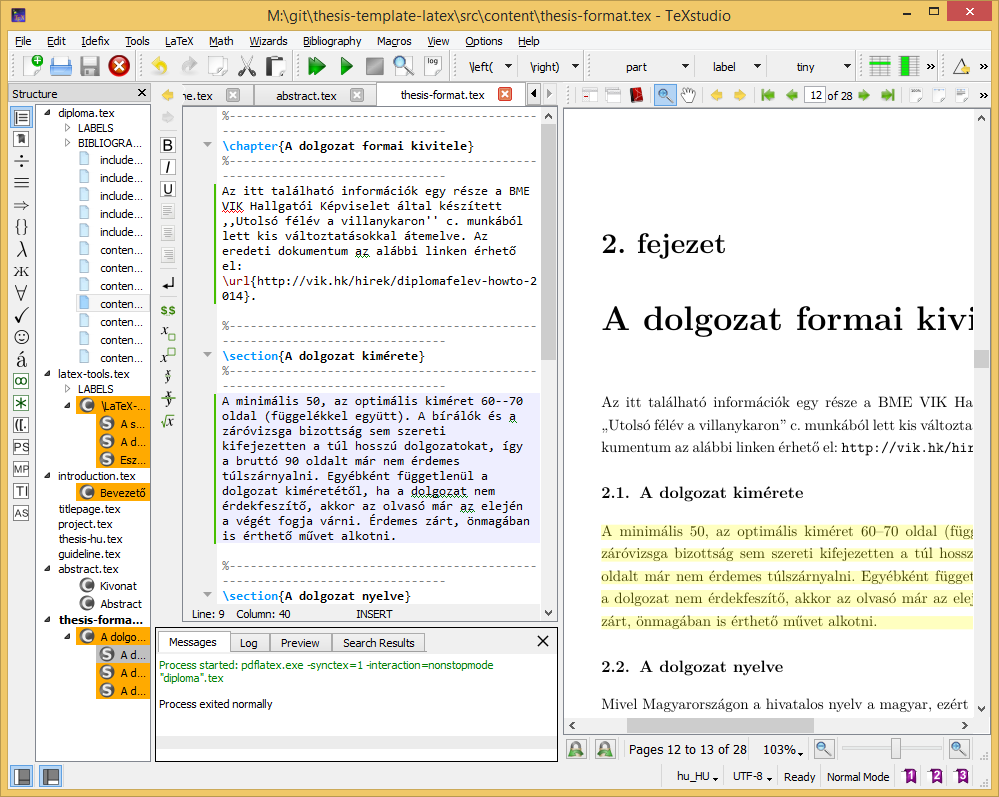
\includegraphics[width=150mm, keepaspectratio]{figures/TeXstudio.png}
\caption{A TeXstudio \LaTeX-szerkesztő.} 
\end{figure}

%----------------------------------------------------------------------------
\clearpage\section{Válasz az ,,Élet, a világmindenség, meg minden'' kérdésére}
%----------------------------------------------------------------------------
A Pitagorasz-tételből levezetve
\begin{align}
c^2=a^2+b^2=42.
\end{align}
A Faraday-indukciós törvényből levezetve
\begin{align}
\rot E=-\frac{dB}{dt}\hspace{1cm}\longrightarrow \hspace{1cm}
U_i=\oint\limits_\mathbf{L}{\mathbf{E}\mathbf{dl}}=-\frac{d}{dt}\int\limits_A{\mathbf{B}\mathbf{da}}=42.
\end{align}


%\label{page:last}
\end{document}
